% Options for packages loaded elsewhere
\PassOptionsToPackage{unicode}{hyperref}
\PassOptionsToPackage{hyphens}{url}
%
\documentclass[
]{book}
\usepackage{lmodern}
\usepackage{amssymb,amsmath}
\usepackage{ifxetex,ifluatex}
\ifnum 0\ifxetex 1\fi\ifluatex 1\fi=0 % if pdftex
  \usepackage[T1]{fontenc}
  \usepackage[utf8]{inputenc}
  \usepackage{textcomp} % provide euro and other symbols
\else % if luatex or xetex
  \usepackage{unicode-math}
  \defaultfontfeatures{Scale=MatchLowercase}
  \defaultfontfeatures[\rmfamily]{Ligatures=TeX,Scale=1}
\fi
% Use upquote if available, for straight quotes in verbatim environments
\IfFileExists{upquote.sty}{\usepackage{upquote}}{}
\IfFileExists{microtype.sty}{% use microtype if available
  \usepackage[]{microtype}
  \UseMicrotypeSet[protrusion]{basicmath} % disable protrusion for tt fonts
}{}
\makeatletter
\@ifundefined{KOMAClassName}{% if non-KOMA class
  \IfFileExists{parskip.sty}{%
    \usepackage{parskip}
  }{% else
    \setlength{\parindent}{0pt}
    \setlength{\parskip}{6pt plus 2pt minus 1pt}}
}{% if KOMA class
  \KOMAoptions{parskip=half}}
\makeatother
\usepackage{xcolor}
\IfFileExists{xurl.sty}{\usepackage{xurl}}{} % add URL line breaks if available
\IfFileExists{bookmark.sty}{\usepackage{bookmark}}{\usepackage{hyperref}}
\hypersetup{
  pdftitle={Laboratório de Sistemas de Controle},
  pdfauthor={Djonathan Luiz de Oliveira Quadras},
  hidelinks,
  pdfcreator={LaTeX via pandoc}}
\urlstyle{same} % disable monospaced font for URLs
\usepackage{color}
\usepackage{fancyvrb}
\newcommand{\VerbBar}{|}
\newcommand{\VERB}{\Verb[commandchars=\\\{\}]}
\DefineVerbatimEnvironment{Highlighting}{Verbatim}{commandchars=\\\{\}}
% Add ',fontsize=\small' for more characters per line
\usepackage{framed}
\definecolor{shadecolor}{RGB}{248,248,248}
\newenvironment{Shaded}{\begin{snugshade}}{\end{snugshade}}
\newcommand{\AlertTok}[1]{\textcolor[rgb]{0.94,0.16,0.16}{#1}}
\newcommand{\AnnotationTok}[1]{\textcolor[rgb]{0.56,0.35,0.01}{\textbf{\textit{#1}}}}
\newcommand{\AttributeTok}[1]{\textcolor[rgb]{0.77,0.63,0.00}{#1}}
\newcommand{\BaseNTok}[1]{\textcolor[rgb]{0.00,0.00,0.81}{#1}}
\newcommand{\BuiltInTok}[1]{#1}
\newcommand{\CharTok}[1]{\textcolor[rgb]{0.31,0.60,0.02}{#1}}
\newcommand{\CommentTok}[1]{\textcolor[rgb]{0.56,0.35,0.01}{\textit{#1}}}
\newcommand{\CommentVarTok}[1]{\textcolor[rgb]{0.56,0.35,0.01}{\textbf{\textit{#1}}}}
\newcommand{\ConstantTok}[1]{\textcolor[rgb]{0.00,0.00,0.00}{#1}}
\newcommand{\ControlFlowTok}[1]{\textcolor[rgb]{0.13,0.29,0.53}{\textbf{#1}}}
\newcommand{\DataTypeTok}[1]{\textcolor[rgb]{0.13,0.29,0.53}{#1}}
\newcommand{\DecValTok}[1]{\textcolor[rgb]{0.00,0.00,0.81}{#1}}
\newcommand{\DocumentationTok}[1]{\textcolor[rgb]{0.56,0.35,0.01}{\textbf{\textit{#1}}}}
\newcommand{\ErrorTok}[1]{\textcolor[rgb]{0.64,0.00,0.00}{\textbf{#1}}}
\newcommand{\ExtensionTok}[1]{#1}
\newcommand{\FloatTok}[1]{\textcolor[rgb]{0.00,0.00,0.81}{#1}}
\newcommand{\FunctionTok}[1]{\textcolor[rgb]{0.00,0.00,0.00}{#1}}
\newcommand{\ImportTok}[1]{#1}
\newcommand{\InformationTok}[1]{\textcolor[rgb]{0.56,0.35,0.01}{\textbf{\textit{#1}}}}
\newcommand{\KeywordTok}[1]{\textcolor[rgb]{0.13,0.29,0.53}{\textbf{#1}}}
\newcommand{\NormalTok}[1]{#1}
\newcommand{\OperatorTok}[1]{\textcolor[rgb]{0.81,0.36,0.00}{\textbf{#1}}}
\newcommand{\OtherTok}[1]{\textcolor[rgb]{0.56,0.35,0.01}{#1}}
\newcommand{\PreprocessorTok}[1]{\textcolor[rgb]{0.56,0.35,0.01}{\textit{#1}}}
\newcommand{\RegionMarkerTok}[1]{#1}
\newcommand{\SpecialCharTok}[1]{\textcolor[rgb]{0.00,0.00,0.00}{#1}}
\newcommand{\SpecialStringTok}[1]{\textcolor[rgb]{0.31,0.60,0.02}{#1}}
\newcommand{\StringTok}[1]{\textcolor[rgb]{0.31,0.60,0.02}{#1}}
\newcommand{\VariableTok}[1]{\textcolor[rgb]{0.00,0.00,0.00}{#1}}
\newcommand{\VerbatimStringTok}[1]{\textcolor[rgb]{0.31,0.60,0.02}{#1}}
\newcommand{\WarningTok}[1]{\textcolor[rgb]{0.56,0.35,0.01}{\textbf{\textit{#1}}}}
\usepackage{longtable,booktabs}
% Correct order of tables after \paragraph or \subparagraph
\usepackage{etoolbox}
\makeatletter
\patchcmd\longtable{\par}{\if@noskipsec\mbox{}\fi\par}{}{}
\makeatother
% Allow footnotes in longtable head/foot
\IfFileExists{footnotehyper.sty}{\usepackage{footnotehyper}}{\usepackage{footnote}}
\makesavenoteenv{longtable}
\usepackage{graphicx}
\makeatletter
\def\maxwidth{\ifdim\Gin@nat@width>\linewidth\linewidth\else\Gin@nat@width\fi}
\def\maxheight{\ifdim\Gin@nat@height>\textheight\textheight\else\Gin@nat@height\fi}
\makeatother
% Scale images if necessary, so that they will not overflow the page
% margins by default, and it is still possible to overwrite the defaults
% using explicit options in \includegraphics[width, height, ...]{}
\setkeys{Gin}{width=\maxwidth,height=\maxheight,keepaspectratio}
% Set default figure placement to htbp
\makeatletter
\def\fps@figure{htbp}
\makeatother
\setlength{\emergencystretch}{3em} % prevent overfull lines
\providecommand{\tightlist}{%
  \setlength{\itemsep}{0pt}\setlength{\parskip}{0pt}}
\setcounter{secnumdepth}{5}
\usepackage{booktabs}
\usepackage[]{natbib}
\bibliographystyle{apalike}

\title{Laboratório de Sistemas de Controle}
\author{Djonathan Luiz de Oliveira Quadras}
\date{2020-07-08}

\usepackage{amsthm}
\newtheorem{theorem}{Teorema}[chapter]
\newtheorem{lemma}{Lema}[chapter]
\newtheorem{corollary}{Corolário}[chapter]
\newtheorem{proposition}{Proposição}[chapter]
\newtheorem{conjecture}{Conjectura}[chapter]
\theoremstyle{definition}
\newtheorem{definition}{Definição}[chapter]
\theoremstyle{definition}
\newtheorem{example}{Exemplo}[chapter]
\theoremstyle{definition}
\newtheorem{exercise}{Exercício}[chapter]
\theoremstyle{remark}
\newtheorem*{remark}{Remark}
\newtheorem*{solution}{Solution}
\begin{document}
\maketitle

{
\setcounter{tocdepth}{1}
\tableofcontents
}
\hypertarget{apresentauxe7uxe3o}{%
\chapter*{Apresentação}\label{apresentauxe7uxe3o}}
\addcontentsline{toc}{chapter}{Apresentação}

Working on it :)

\hypertarget{simulauxe7uxe3o-de-sistemas}{%
\chapter{Simulação de Sistemas}\label{simulauxe7uxe3o-de-sistemas}}

Este laboratório consistiu apenas na apresentação da disciplina, da ferramenta e do método que será aplicado. Não teve nehuma atividade desenvolvida.

\hypertarget{lab2}{%
\chapter{Efeitos de Pólos e Zeros na Dinâmica}\label{lab2}}

Nesta experiência, verificaremos a influência dos pólos e zeros de uma Função de Transferência na resposta dinâmica para entradas do tipo degrau e também para entradas senoidais. Utilizaremos o Matlab para realizar as
simulações.

\hypertarget{puxf3los-e-zeros}{%
\section{Pólos e Zeros}\label{puxf3los-e-zeros}}

Considere uma função de Trasnferência da forma

\[
G(s) = \frac{Y(s)}{U(s)} = \frac{N(s)}{D(s)} = \frac{b_1s^m +b_2s^{m-1} + \dots + b_ms + b_{m+1}}{s^n + a_1s^{n-1}+ \dots + a_{n-1}s + a_n}
\]

onde \(Y(s)\) é a saída, \(U(s)\) é a entrada, \(n \geq m\) e todos os coeficientes são reais. Temos as seguintes definições:

\begin{enumerate}
\def\labelenumi{\arabic{enumi}.}
\tightlist
\item
  Os pólos \(G(s)\) são as raízes de \(D(s)\) (\(D(s) = 0\));
\item
  Os \emph{zeros} de \(G(s)\) são as raízes de \(N(s)\) (\(N(s) = 0\));
\item
  \(G(s)\) é \emph{estável} quando todos os pólos possuem parte real negativa, ou seja, estão no semi-plano esquerdo (SPE) do plano \(s\);
\item
  \(G(s)\) é \emph{instável} quando existe ao menos um pólo com parte real positiva, ou seja, no semi-plano (SPD);
\item
  \(G(s)\) é de \emph{fase não-mínima} quando há pólos ou zeros no SPE.
\end{enumerate}

Considere que \(G(s)\) é estável, ou seja, todos os pólos estão no SPE. Em geral, para entradas do tipo degrau, temos:

\begin{enumerate}
\def\labelenumi{\arabic{enumi}.}
\tightlist
\item
  A componente da resposta dinâmica referente a um pólo afastado da origem (do plano \(s\)) é relativamente rápida;
\item
  A componente da resposta dinâmica referente a um pólo próximo da origem é relativamente lenta;
\item
  Um zero tende a fazer com que a resposta dinâmica apresente sobressinal. Quanto mais próximo da origem estiver o zero, maior o sobressinal. E, quanto mais longe da origem, menor se torna o sobressinal, podendo o mesmo não existir. Assim, um sistema de segunda ordem com pólos reais e um zero poderá apresentar um sobressinal dependendo do posicionamento do zero no plano \(s\);
\item
  Um zero bem próximo de um pólo tende a anular os efeitos dos mesmos na resposta dinâmica.
\end{enumerate}

\hypertarget{problemas-laboratuxf3rio-2}{%
\chapter*{Problemas Laboratório 2}\label{problemas-laboratuxf3rio-2}}
\addcontentsline{toc}{chapter}{Problemas Laboratório 2}

Estes problemas são relacionados ao assunto abordado no Laboratório \ref{lab2}.

\hypertarget{problema-2.1}{%
\section*{Problema 2.1}\label{problema-2.1}}
\addcontentsline{toc}{section}{Problema 2.1}

Considere o sistema de primeira ordem
\[
G(s) = \frac{1}{\tau s +1},
\]
onde \(\tau = 1\), \(\tau = 0.5\). Para cada valor de \(\tau\), determine o pólo e sua posição no plano \(s\) (use os comandos \texttt{zpk} e \texttt{pzmap} no Matlab), e conclua sobre a estabilidade e a rapidez da resposta do sistema. Simule para uma entrada do tipo degrau unitário. Analise e compare os resultados. Agora, repita o procedimento para o sistema
\[
G(s) = \frac{1}{s-1}.
\]

\hypertarget{resoluuxe7uxe3o}{%
\subsubsection*{Resolução}\label{resoluuxe7uxe3o}}
\addcontentsline{toc}{subsubsection}{Resolução}

A resolução será feita em quatro partes: (1) a resolução para \(\tau = 1\) usando \texttt{pzmap}, (2) a resolução para \(\tau = 0.5\) usando \texttt{pzmap}, (3) a simulação e comparação dos resultados e, por fim, (4) a resolução para \(G(s) =\frac {1}{s-1}\).

\hypertarget{parte-1}{%
\paragraph*{Parte 1}\label{parte-1}}
\addcontentsline{toc}{paragraph}{Parte 1}

Para \(\tau = 1\), temos a função de transferência dada por
\[
G(S)= \frac {1}{s+1}.
\]

O código implementado no \texttt{Matlab} foi o apresentado abaixo.

\begin{Shaded}
\begin{Highlighting}[]
\VariableTok{g} \OperatorTok{=} \VariableTok{tf}\NormalTok{([}\FloatTok{1}\NormalTok{]}\OperatorTok{,}\NormalTok{ [}\FloatTok{1} \FloatTok{1}\NormalTok{])}
\NormalTok{[}\VariableTok{p}\OperatorTok{,} \VariableTok{z}\NormalTok{] }\OperatorTok{=} \VariableTok{pzmap}\NormalTok{(}\VariableTok{g}\NormalTok{)}
\VariableTok{pzmap}\NormalTok{(}\VariableTok{g}\NormalTok{)}
\end{Highlighting}
\end{Shaded}

Tendo como resultados de pólos e zeros:

\begin{verbatim}
p =

    -1


z =

  0×1 empty double column vector
\end{verbatim}

Ou seja, a função de transferência não apresenta zeros e tem seu pólo em \(s = -1\). A sua posição no plano é apresentada na figura abaixo.

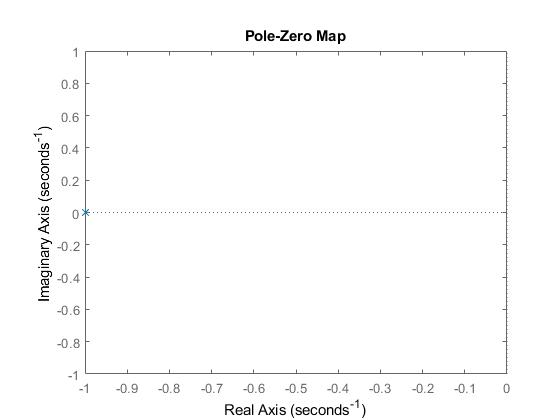
\includegraphics{Imagens/Lab2/tau1.jpg}

Como o pólo da função de transferência se encontra na SPE, conclui-se que o sistema se compartará de uma forma estável.

\hypertarget{parte-2}{%
\paragraph*{Parte 2}\label{parte-2}}
\addcontentsline{toc}{paragraph}{Parte 2}

Para \(\tau = 0.5\), temos a função de transferência dada por
\[
G(S)= \frac {1}{0.5s+1}.
\]

O código implementado no \texttt{Matlab} foi o apresentado abaixo.

\begin{Shaded}
\begin{Highlighting}[]
\VariableTok{g} \OperatorTok{=} \VariableTok{tf}\NormalTok{([}\FloatTok{1}\NormalTok{]}\OperatorTok{,}\NormalTok{ [}\FloatTok{0.5} \FloatTok{1}\NormalTok{])}
\NormalTok{[}\VariableTok{p}\OperatorTok{,} \VariableTok{z}\NormalTok{] }\OperatorTok{=} \VariableTok{pzmap}\NormalTok{(}\VariableTok{g}\NormalTok{)}
\VariableTok{pzmap}\NormalTok{(}\VariableTok{g}\NormalTok{)}
\end{Highlighting}
\end{Shaded}

Tendo como resultados de pólos e zeros:

\begin{verbatim}
p =

    -2


z =

  0×1 empty double column vector
\end{verbatim}

Ou seja, a função de transferência não apresenta zeros e tem seu pólo em \(s = -2\). A sua posição no plano é apresentada na figura abaixo

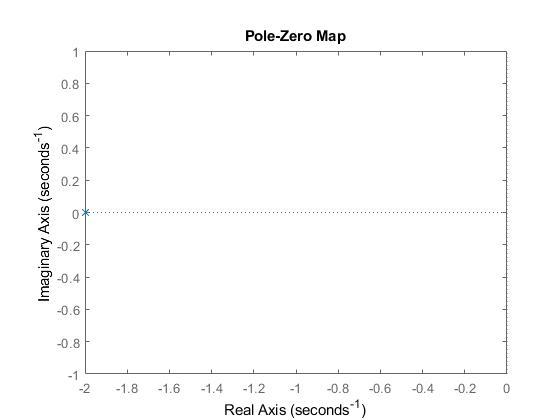
\includegraphics{Imagens/Lab2/tau2.jpg}

Como o pólo da função de transferência se encontra na SPE, conclui-se que o sistema se compartará de uma forma estável. Também é possível concluir que o sistema alcanraça a estabilidade mais rápido para \(\tau = 0.5\).

\hypertarget{parte-3}{%
\paragraph*{Parte 3}\label{parte-3}}
\addcontentsline{toc}{paragraph}{Parte 3}

A simulação do sistema implementada em \texttt{Matlab} está apresentado na figura abaixo.

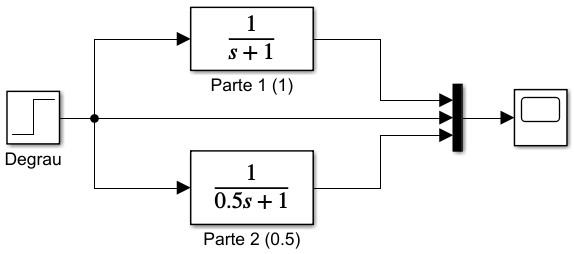
\includegraphics{Imagens/Lab2/sim1.jpg}

O resultado apresentado pelo \emph{scope} é apresentado na figura abaixo.

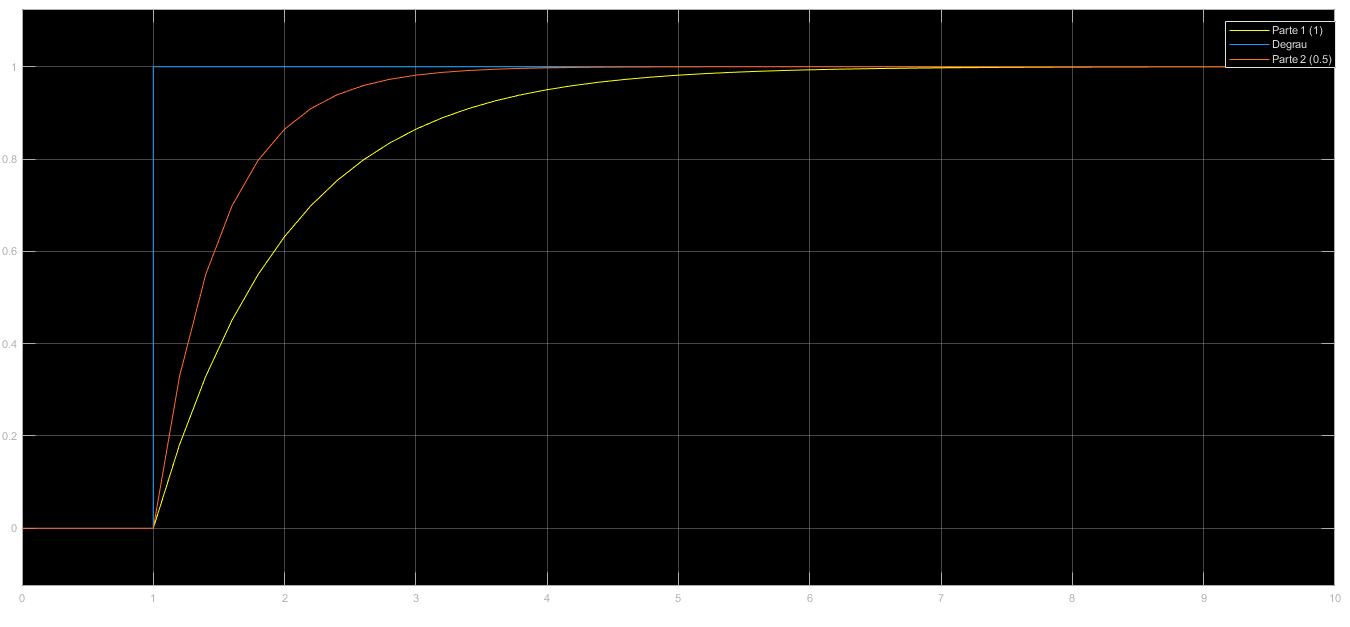
\includegraphics{Imagens/Lab2/resultSim1.jpg}

Percebe-se que, assim como esperado, o sistema se comporta de forma estável e tem uma convergência mais rápida para \(\tau = 0.5\).

\hypertarget{parte-4}{%
\paragraph*{Parte 4}\label{parte-4}}
\addcontentsline{toc}{paragraph}{Parte 4}

Para a última etapa temos a função de transferência dada por
\[
G(S)= \frac {1}{s-1}.
\]

O código implementado no \texttt{Matlab} foi o apresentado abaixo.

\begin{Shaded}
\begin{Highlighting}[]
\VariableTok{g} \OperatorTok{=} \VariableTok{tf}\NormalTok{([}\FloatTok{1}\NormalTok{]}\OperatorTok{,}\NormalTok{ [}\FloatTok{1} \OperatorTok{{-}}\FloatTok{1}\NormalTok{])}
\NormalTok{[}\VariableTok{p}\OperatorTok{,} \VariableTok{z}\NormalTok{] }\OperatorTok{=} \VariableTok{pzmap}\NormalTok{(}\VariableTok{g}\NormalTok{)}
\VariableTok{pzmap}\NormalTok{(}\VariableTok{g}\NormalTok{)}
\end{Highlighting}
\end{Shaded}

Tendo como resultados de pólos e zeros:

\begin{verbatim}
p =

    1


z =

  0×1 empty double column vector
\end{verbatim}

Ou seja, a função de transferência não apresenta zeros e tem seu pólo em \(s = 1\). A sua posição no plano é apresentada na figura abaixo

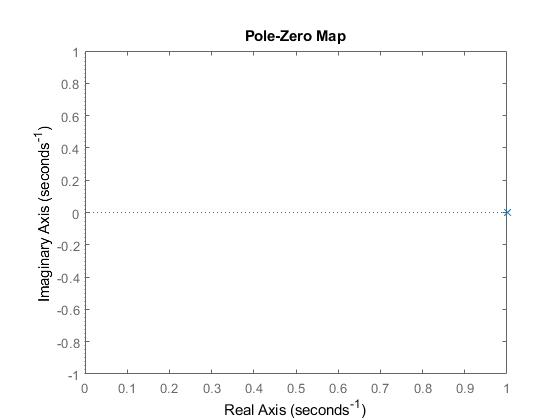
\includegraphics{Imagens/Lab2/tau3.jpg}

Como o pólo da função de transferência se encontra na SPD, conclui-se que o sistema se compartará de uma forma instável. A simulação em \texttt{Matlab} está apresentada na figura abaixo.

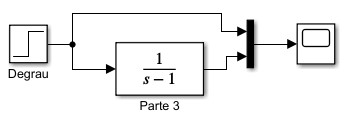
\includegraphics{Imagens/Lab2/sim2.jpg}

O resultado apresentado pelo \emph{scope} é apresentado na figura abaixo.

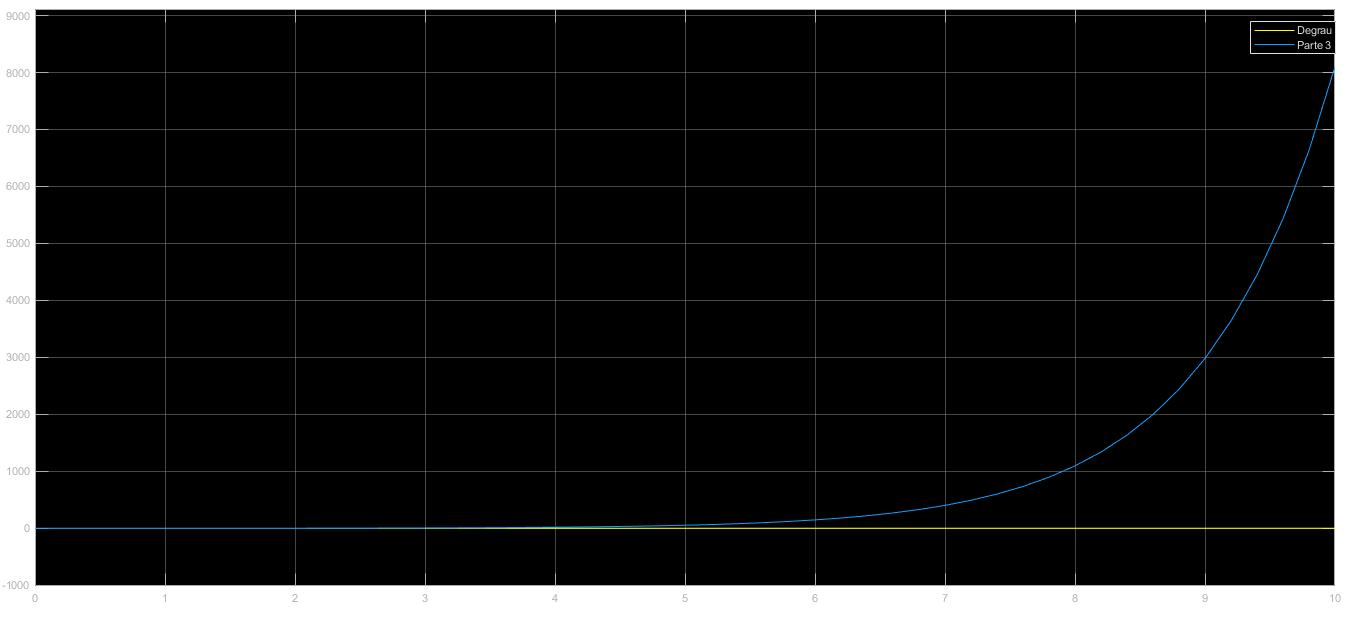
\includegraphics{Imagens/Lab2/resultSim2.jpg}

O resultado comprova o esperado. O sistema se comporta de forma instável para a função de transferência dada por \(G(s) = \frac {1}{s-1}\).

\hypertarget{problema-2.2}{%
\section*{Problema 2.2}\label{problema-2.2}}
\addcontentsline{toc}{section}{Problema 2.2}

Considere o sistema de primeira ordem (integrador)
\[
G(s) = \frac {1}{s}.
\]

Determine o pólo e a sua posição no plano \(s\) e simule para uma entrada do tipo degrau unitário e também para \(\sin {(t)}\) (para \(\sin {(t)}\), escolha \textbf{Max Step Size = 0.1} em \textbf{Simulation \(\implies\) Configurarion Parameters}). Note que a saída é a integral da entrada. Tais resultados eram esperados? Dica: relembre que \(Y(s) = G(s)U(s)\), e que se \(x(t) \iff X(S)\), então \(\int_0^t x(\tau) \mathrm{d}\tau \iff X(s)/s\).

\hypertarget{resoluuxe7uxe3o-1}{%
\subsubsection*{Resolução}\label{resoluuxe7uxe3o-1}}
\addcontentsline{toc}{subsubsection}{Resolução}

O código utilizado no \texttt{Matlab} é apresentado abaixo.

\begin{Shaded}
\begin{Highlighting}[]
\VariableTok{g} \OperatorTok{=} \VariableTok{tf}\NormalTok{([}\FloatTok{1}\NormalTok{]}\OperatorTok{,}\NormalTok{ [}\FloatTok{1} \FloatTok{0}\NormalTok{])}
\NormalTok{[}\VariableTok{p}\OperatorTok{,}\VariableTok{z}\NormalTok{] }\OperatorTok{=} \VariableTok{pzmap}\NormalTok{(}\VariableTok{g}\NormalTok{)}
\VariableTok{pzmap}\NormalTok{(}\VariableTok{g}\NormalTok{)}
\end{Highlighting}
\end{Shaded}

Obtendo como resultado:

\begin{verbatim}
p =

     0


z =

  0×1 empty double column vector
\end{verbatim}

Conclue-se então que a função de transferência \(G(s) = \frac {1}{s}\) não tem zeros e tem pólo em \(s = 0\). O mapa da posição no plano é mostrado na figura abaixo.

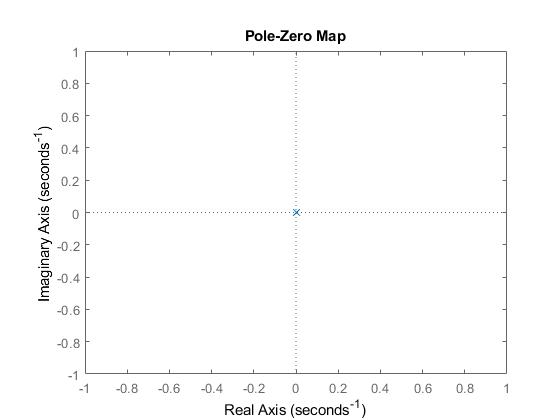
\includegraphics{Imagens/Lab2/prob2.jpg}

Isso mostra que o sistema é um caso crítico. Neste caso a resposta em regime permanente do sistema a uma entrada de amplitude limitada será uma senóide.

A simulação feita em \texttt{Matlab} está apresentada na figura abaixo.

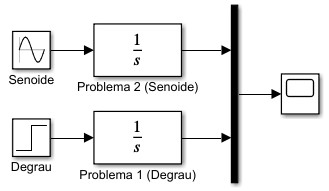
\includegraphics{Imagens/Lab2/simP2.jpg}

O resultado da simulação é apresentado na figura abaixo.

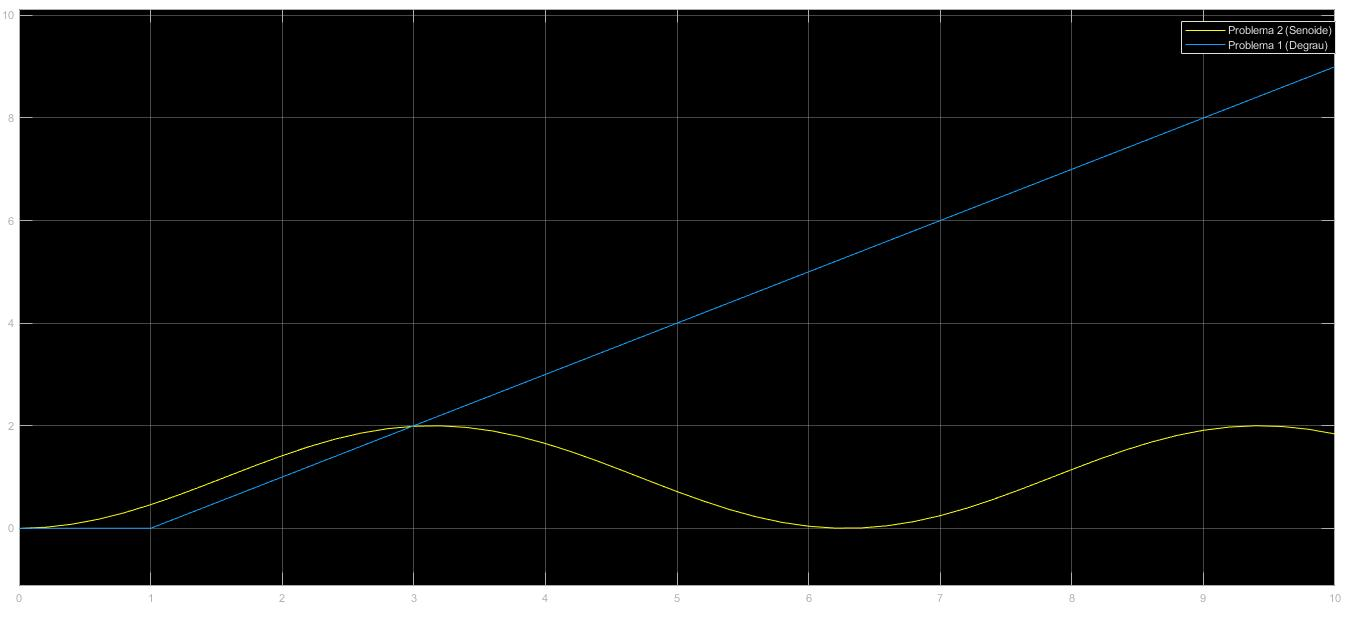
\includegraphics{Imagens/Lab2/prob2B.jpg}

O resultados eram esperados, uma vez que em um estado crítico a função de transferência pode estar em um estado permanente senoidal caso a entrada seja senoidal ou pode divergir caso a entrada seja um sinal constante.

\hypertarget{problema-2.3}{%
\section*{Problema 2.3}\label{problema-2.3}}
\addcontentsline{toc}{section}{Problema 2.3}

Considere o sistema de segunda ordem
\[
G(s) = \frac {1}{s^2 +25}.
\]

Determine os pólos e suas posições no plano \(s\). Simule para as seguintes entradas: degrau unitário, \(\sin (4t)\), \(\sin(6t)\). Observe que a saída é limitada. Agora, semule para a entrada \(\sin(5t)\). Note que a amplitude de saída cresce indefinidamente. Tal fenômeno é denominado de \emph{ressonância}. De moro mais geral, para
\[
G(s) = \frac {1}{s^2+\omega_0^2},
\]
teremos ressonância quando aplicamos uma entrada senoidal da forma \(\sin(\omega_0t + \phi)\). Note que a \emph{frequência de ressonância} \(\omega_0\) é igual a parte imaginária dos pólos de \(G(s)\).

\hypertarget{resoluuxe7uxe3o-2}{%
\subsubsection*{Resolução}\label{resoluuxe7uxe3o-2}}
\addcontentsline{toc}{subsubsection}{Resolução}

O código utilizado no \texttt{Matlab} é apresentado abaixo.

\begin{Shaded}
\begin{Highlighting}[]
\VariableTok{g} \OperatorTok{=} \VariableTok{tf}\NormalTok{([}\FloatTok{1}\NormalTok{]}\OperatorTok{,}\NormalTok{ [}\FloatTok{1} \FloatTok{0} \FloatTok{25}\NormalTok{])}
\NormalTok{[}\VariableTok{p}\OperatorTok{,}\VariableTok{z}\NormalTok{] }\OperatorTok{=} \VariableTok{pzmap}\NormalTok{(}\VariableTok{g}\NormalTok{)}
\VariableTok{pzmap}\NormalTok{(}\VariableTok{g}\NormalTok{)}
\end{Highlighting}
\end{Shaded}

Obtendo como resultado:

\begin{verbatim}
p =

   0.0000 + 5.0000i
   0.0000 - 5.0000i


z =

  0×1 empty double column vector
\end{verbatim}

Conclue-se então que a função de transferência \(G(s) = \frac {1}{s^2 +25}\) não tem zeros e tem pólo em \(s = \pm 5i\). O mapa da posição no plano é mostrado na figura abaixo.

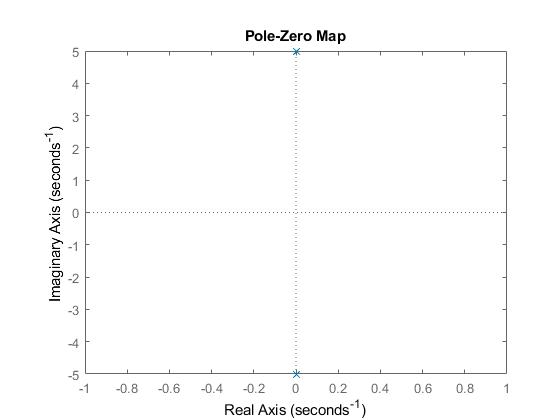
\includegraphics{Imagens/Lab2/prob3.jpg}

De acordo com o mapa de posição, pode-se concluir que a função de transferência é classificada como um caso crítico. A figura abaixo apresenta o modelo de simulação criado no \texttt{Simulink}.

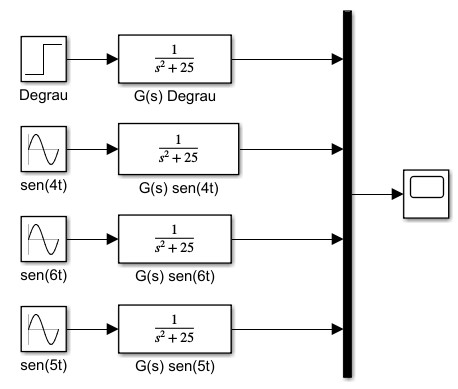
\includegraphics{Imagens/Lab2/modelSim3.jpg}

O resultado da simulação é apresentado abaixo.

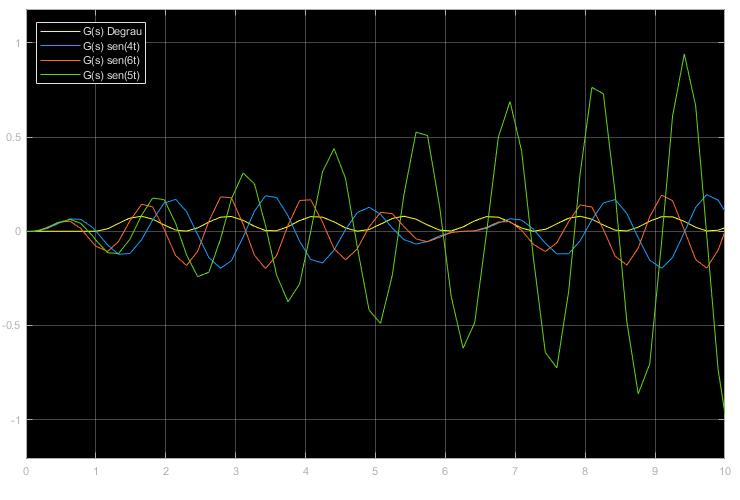
\includegraphics{Imagens/Lab2/prob3Sim.jpg}

É fácil perceber que o modelo se comporta de maneira instável com a entrada \(u(t) = \sin(5t)\), se mostrando estável nas demais situações.

\hypertarget{problema-2.4}{%
\section*{Problema 2.4}\label{problema-2.4}}
\addcontentsline{toc}{section}{Problema 2.4}

Considere o sistema de segunda orde
\[
G(s) = \frac {1.6}{(s+1)(s+2)} = \frac {0.8}{0.5s^2+1.5s+1}.
\]

Determine os pólos e suas posições no plano \(s\) e simule para uma entrada do tipo degrau unitário. Note que não há sobressinal. Tal resultado era esperado? Justifique.

Agora, adicionando um zero, temos
\[
G(s) = \frac {1.6(\beta s+1)}{(s+1)(s+2)} = \frac {0.8(\beta s+1)}{0.5s^2 +1.5s +1},
\]
onde \(\beta = 0.1\), \(\beta = 0.6\), \(\beta = 0.99\), \(\beta = 1.2\), \(\beta = 2\), \(\beta = 10\). Para cada valor de \(\beta\), determine os pólos e zeros, suas posições no plano \(s\) e simule para uma entrada do tipo degrau unitário. Analise e compare os resultados. Note que dependendo da posição do zero o sobressinal será maior ou menor, podendo também não estar presente.

\hypertarget{resoluuxe7uxe3o-3}{%
\subsubsection*{Resolução}\label{resoluuxe7uxe3o-3}}
\addcontentsline{toc}{subsubsection}{Resolução}

Utilizando a função \texttt{pzmap()} do \texttt{Matlab} para encontrar os pólos da função de transferência \(G(s) = \frac {0.8}{0.5s^2+1.5s+1}\) temos que a função não possui zeros e possui pólos para \(s = -2\) e \(s = -1\). O mapa de posições é apresentado na figura abaixo.

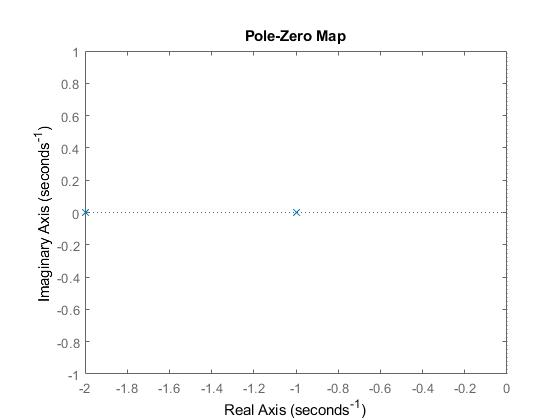
\includegraphics{Imagens/Lab2/prob4.jpg}

O resultado da função de transferência é apresentado na figura abaixo.

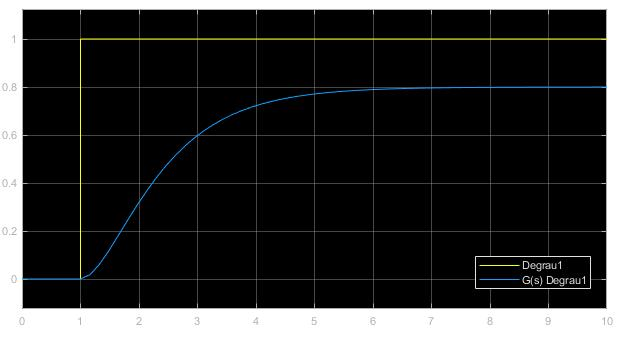
\includegraphics{imagens/Lab2/prob41.jpg}

O resultado não era esperado pois, para uma Função de Transferência de segundo grau é esperado que a resposta tenha sobressinal. Agora, considerando a função de transferência
\[
G(s) = \frac {0.8(\beta s+1)}{0.5s^2+1.5s+1},
\]
e substituindo os valores de \(\beta\) pelos valores propostos temos os valores de zero e pólo apresentados na tabela abaixo.

\begin{table}

\caption{\label{tab:unnamed-chunk-6}Valores de Pólo e Zero variando $\beta$}
\centering
\begin{tabular}[t]{lll}
\toprule
  & Pólos & Zeros\\
\midrule
$\beta = 0.1$ & {-2, -1} & -10.0\\
$\beta = 0.6$ & {-2, -1} & -1.67\\
$\beta = 0.99$ & {-2, -1} & -1.01\\
$\beta = 1.2$ & {-2, -1} & -0.83\\
$\beta = 2$ & {-2, -1} & -0.50\\
\addlinespace
$\beta = 10$ & {-2, -1} & -0.10\\
\bottomrule
\end{tabular}
\end{table}

Os gráficos de posição estão apresentados abaixo.

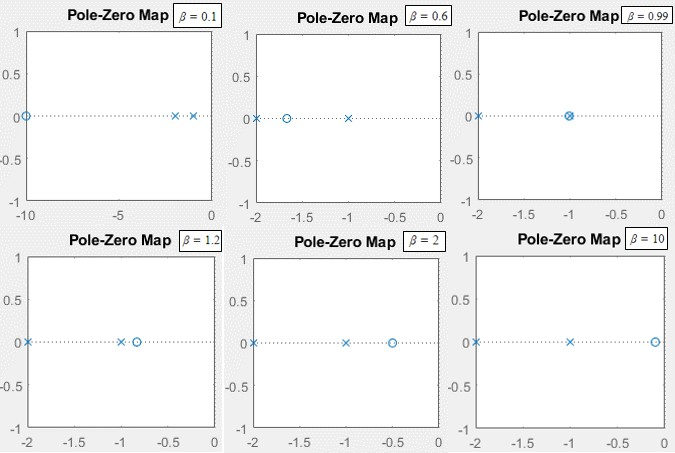
\includegraphics{Imagens/Lab2/prob4Varios.jpg}

A simulação feita em \texttt{Matlab} está apresentada na figura abaixo.

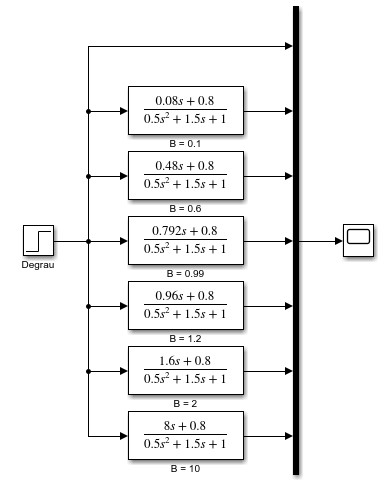
\includegraphics{Imagens/Lab2/modelSim4.jpg}

O resultado da simulação está apresentado na figura abaixo.

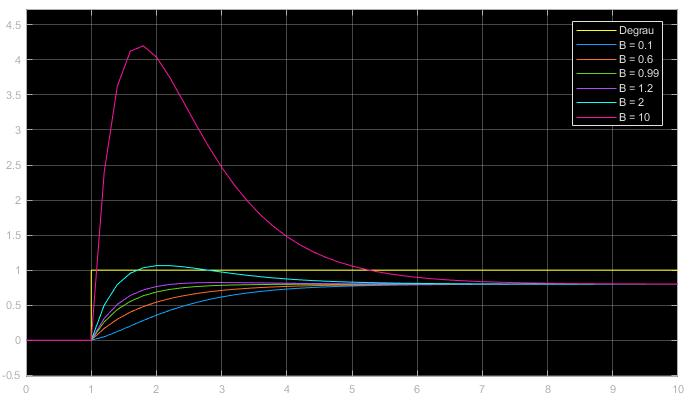
\includegraphics{Imagens/Lab2/prob4SimResult.jpg}

É possível perceber que quanto mais alto o valor de \(\beta\) maior o sobressinal. Também é possível perceber que há um intervalo no qual o tempo de reação aumenta, encontrando seu tempo de reação mínimo, voltando então a aumentar.

\hypertarget{problema-2.5}{%
\section*{Problema 2.5}\label{problema-2.5}}
\addcontentsline{toc}{section}{Problema 2.5}

Considere o sistema de segunda ordem
\[
G(s) = \frac {0.9}{s^2+s+1}.
\]

Determine os pólos e suas posições no plano \(s\) e simule para uma entrada do tipo degrau unitário. Note que há sobressinal. Tal resultado era esperado? Justifique.

Agora, adicionando um zero, temos
\[
G_z(s) = \frac {0.9(\beta s+1)}{s^2+s+1},
\]
onde \(\beta = 0.05\), \(\beta = 0.5\), \(\beta = 1\) e \(\beta = 2.5\). Para cada valor de \(\beta\) determine os pólos e zeros, suas posições no plano \(s\) e simule para uma entrada do tipo degrau unitário. Analise e compare os resultados.

\hypertarget{resoluuxe7uxe3o-4}{%
\subsubsection*{Resolução}\label{resoluuxe7uxe3o-4}}
\addcontentsline{toc}{subsubsection}{Resolução}

Utilizando a função \texttt{pzmap()} do \texttt{Matlab} para encontrar os pólos da função de transferência \(G(s) = \frac {0.9}{s^2+s+1}\) temos que a função não possui zeros e possui pólos para \(s = -0.5 + 0.86i\) e \(s = -0.5 -0.86i\). O mapa de posições é apresentado na figura abaixo.

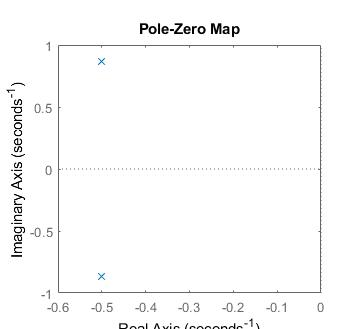
\includegraphics{Imagens/Lab2/prob5.jpg}

O resultado da função de transferência é apresentado na figura abaixo.

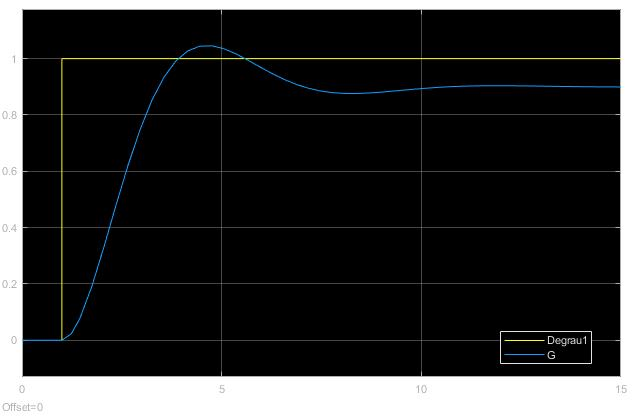
\includegraphics{imagens/Lab2/prob5Sim.jpg}

É possível perceber que há sobressinal.

Agora, considerando a função de transferência \(G_z(s) = \frac {0.9(\beta s+1)}{s^2+s+1}\), e substituindo os valores de \(\beta\) pelos valores propostos temos os valores de zero e pólo apresentados na tabela abaixo.

\begin{table}

\caption{\label{tab:unnamed-chunk-7}Valores de Pólo e Zero variando $\beta$}
\centering
\begin{tabular}[t]{lll}
\toprule
  & Pólos & Zeros\\
\midrule
$\beta = 0.05$ & {$-0.5 \pm 0.86i$} & -20.0\\
$\beta = 0.5$ & {$-0.5 \pm 0.86i$} & -2.0\\
$\beta = 1$ & {$-0.5 \pm 0.86i$} & -1.0\\
$\beta = 2.5$ & {$-0.5 \pm 0.86i$} & -0.4\\
\bottomrule
\end{tabular}
\end{table}

Os gráficos de posição estão apresentados abaixo.

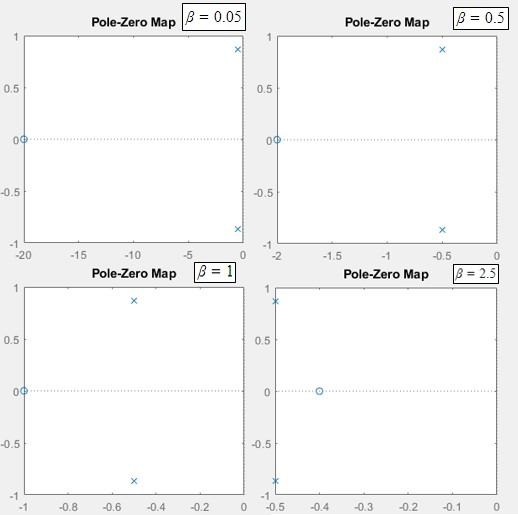
\includegraphics{Imagens/Lab2/prob5Varios.jpg}

A simulação feita em \texttt{Matlab} está apresentada na figura abaixo.

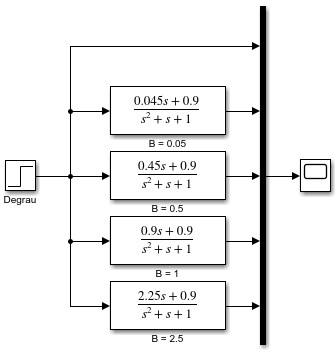
\includegraphics{Imagens/Lab2/modelSim5.jpg}

O resultado da simulação está apresentado na figura abaixo.

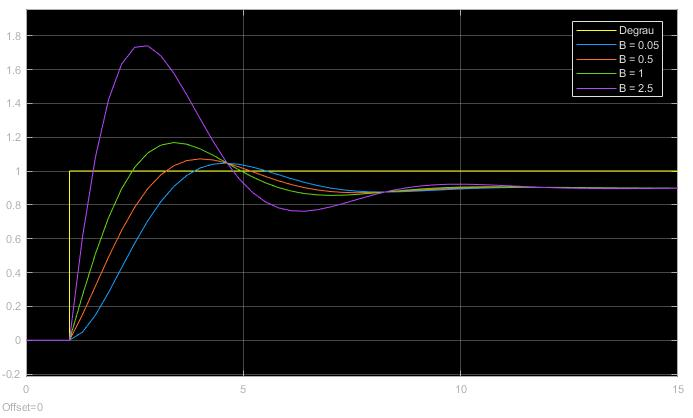
\includegraphics{Imagens/Lab2/prob5SimResult.jpg}

É possível perceber que quanto mais alto o valor de \(\beta\) maior o sobressinal e o tempo de resposta do sistema.

\hypertarget{problema-2.6}{%
\section*{Problema 2.6}\label{problema-2.6}}
\addcontentsline{toc}{section}{Problema 2.6}

Considere o sistema de segunda ordem de fase não-mínima
\[
G(s) = \frac {-s+1}{0.5s^2+1.5s+1}.
\]

Determine os pólos e o zero, suas posições no plano \(s\) e simule para uma entrada do tipo degrau unitário. Note que a resposta é negativa nos instantes iniciais. Justificaremos tal comportamento no que se segue.

Escrevemos
\[
G(s) = \frac {-s+1}{0.5s^2+1.5s+1} = \overbrace{\frac {1}{0.5s^2+1.5s+1}}^{G_1(s)} - \overbrace{\frac {s}{0.5s^2+1.5s+1}}^{G_2(s) = sG_1(S)}.
\]

Assim,
\[
Y(s) = G(s)U(s) = G_1(s)U(s)-G_2(s)U(s) = \underbrace{G_1(s)U(s)}_{Y_1(s)} - \underbrace{sG_1(s)U(s)}_{Y_2(s) = sY_1(s)}.
\]

Relembre-se que se \(x(t) \iff X(S)\) com \(x(0) = 0\), então \(dx(t)/dt \iff sX(s)\). Portanto,
\[
y(t) = y_1(t)-y_2(t)=y_1(t)- \frac {dy_1(t)}{dt}.
\]

Verifique a validade da equação acima no Simulink (utilize o bloco \textbf{Derivative} no Simulink) para uma entrada do tipo degrau unitário. Analise o motivo da resposta ser negativa nos instantes iniciais.

\hypertarget{resoluuxe7uxe3o-5}{%
\subsubsection*{Resolução}\label{resoluuxe7uxe3o-5}}
\addcontentsline{toc}{subsubsection}{Resolução}

Utilizando a função \texttt{pzmap()} do \texttt{Matlab} para encontrar os pólos da função de transferência \(G(s) = \frac {-s +1}{0.5s^2+1.5s+1}\) temos que a função possui zeros para \(s=1\) e possui pólos para \(s = -2\) e \(s = -1\). O mapa de posições é apresentado na figura abaixo.

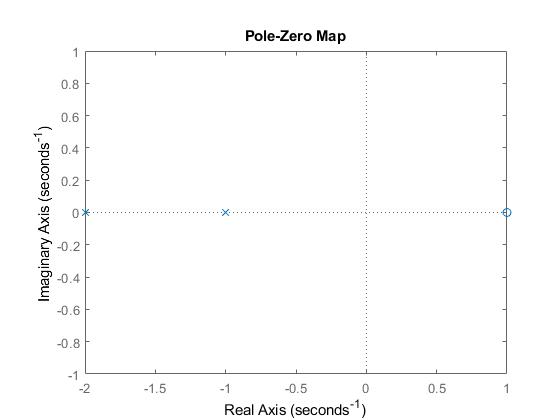
\includegraphics{Imagens/Lab2/prob6A.jpg}

A resposta de \(G(s)\) a uma função degrau unitário é apresentada na figura abaixo.

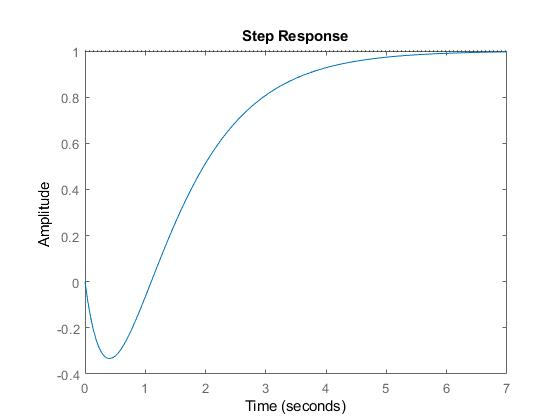
\includegraphics{Imagens/Lab2/prob6B.jpg}

A validade da equação proposta pelo programa é apresentada na figura abaixo. Pode-se perceber que a equação é valida pois as curvas são satisfatoriamente similares.

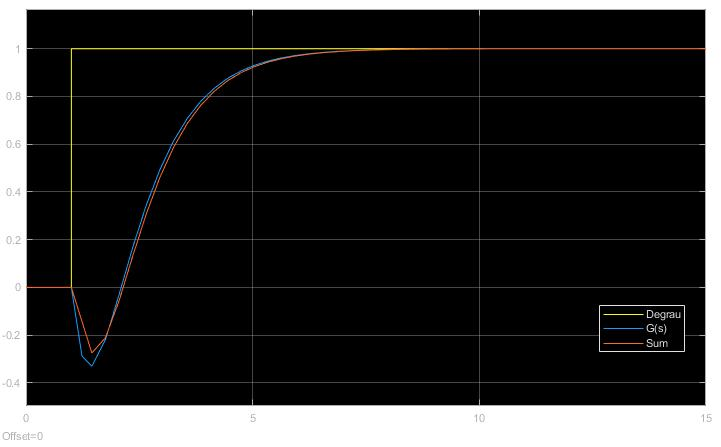
\includegraphics{Imagens/Lab2/prob6C.jpg}

O motivo da resposta ser negativa se deve ao fato de o zero da função \(G(s)\) se encontrar no SPD.

\hypertarget{lab3}{%
\chapter{Identificação de Sistemas}\label{lab3}}

Nesta experiência, veremos como modelar matematicamente um sistema linear por uma Função de Transferência. Identificaremos os parâmetros de uma Função de Transferência de primeira e de segunda ordem. Compararemos a dinâmica do sistema com a do modelo matemático.

\hypertarget{modelagem-de-sistemas-lineares}{%
\section{Modelagem de Sistemas Lineares}\label{modelagem-de-sistemas-lineares}}

Encontrar um modelo matemático que capture as características dinâmicas relevantes de um sistema real é de fundamental importância para a análise e controle do sistema. No Laboratório 1 estudamos um modelo linear com motor CC. Tal modelo pode ser obtido a partir das leis da física (mecânica e eletromagnetismo) e os valores dos parâmetros dependem de constantes e coeficientes físicos (indutância do enrolamento, resistência do enrolamento, constante de torque do motor, coeficiente de atrito ciscoso). Em situações reais, não conheceremos uma estimativa para os mesmos. Por exemplo, todo resistor possui um valor normal e uma faixa de tolerância percentual (e.g.~\(R = 100 \Omega \pm 5\%\)). Além disso, muitas vezes a determinação de um modelo matemático para um sistema a partir de leis naturais é extremamente difícil e, mesmo no caso em que isso é possível, o modelo obtido pode ser demasiadamente complexo para ser estudado matematicamente.

Devido às dificuldades que acabamos de expor, em geral buscamos um modelo matemático relativamente simples mas que capture, ao menos aproximadamente, as características dinâmicas relevantes do sistema. Assim, primeiramente fixamos um modelo (\emph{modelagem} do sistema) e em seguida determinamos de maneira aproximada o valor de seus parâmetros (\emph{identificação} dos parâmetros).

Nesta experiência, consideraremos apenas sistemas lineares que possam ser modelados por uma função de Transferência \(G(s)\) de primeira ordem ou de segunda ordem. Veremos então como identificar os parâmetros de \(G(s)\).

\hypertarget{identificauxe7uxe3o-de-sistemas-de-primeira-ordem}{%
\section{Identificação de sistemas de primeira ordem}\label{identificauxe7uxe3o-de-sistemas-de-primeira-ordem}}

Toda Função de Transferência \(G(s)\) de primeira ordem pode ser escrita na forma padrão como

\begin{align}
G(s) = \frac{K}{\tau s+1}. \label{eq:eq31}
\end{align}

Supunha que \(G(s)\) é estável, ou seja, \(\tau > 0\). considere uma entrada \(u(t) = A\) do tipo degrau de magnitude \(A\). Temos que a saída correspondente é
\[
y(t) = AK(1- e^{\frac {-t}{\tau}}).
\]

O valor da saída em regime permanente é
\[
y(\infty) = AK,
\]
e o tempo de acomodação de \(5\%\) é dado por
\[
0.95KA = KA(1- e^{\frac {-t_s(5\%)}{\tau}}) \implies t_s(5\%) =3 \tau.
\]

Isto é ilustrado na figura 1.

\begin{figure}
\centering
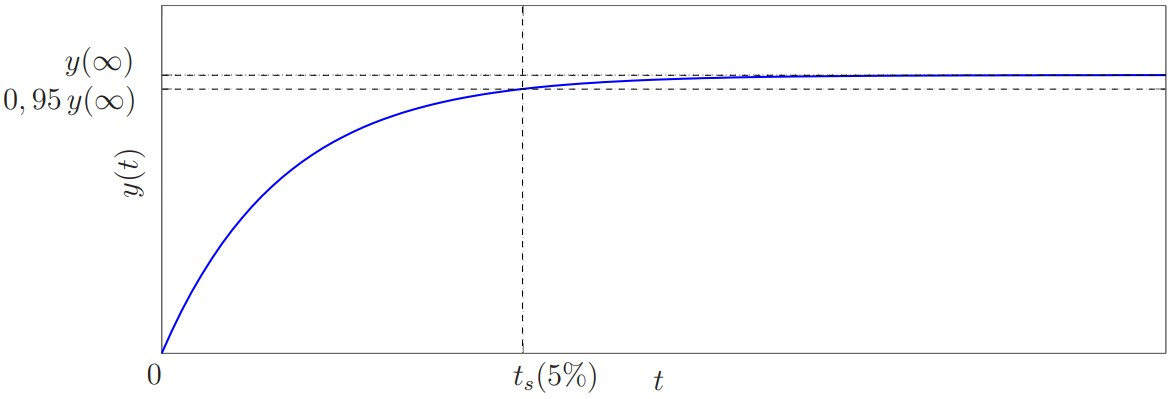
\includegraphics{Imagens/Lab3/Explicação/fig1.jpg}
\caption{Figura 1: Resposta de um sistema de primeira ordem ao degrau.}
\end{figure}

Logo,

\begin{align}
K = \frac{y(\infty)}{A},  \tau = \frac {t_s(5\%)}{3}. \label{eq:eq32}
\end{align}

\hypertarget{identificauxe7uxe3o-de-sistemas-de-segunda-ordem}{%
\section{Identificação de Sistemas de Segunda Ordem}\label{identificauxe7uxe3o-de-sistemas-de-segunda-ordem}}

Toda Função de Transferência \(G(s)\) de segunda ordem com pólos não-nulos pode ser escrita como

\begin{align}
G(s) = \frac {K \omega_n^2}{s^2+2\xi \omega_n+ \omega_n^2}, \label{eq:eq33}
\end{align}

onde \(\omega_n > 0\). Os pólos de \(G(s)\) são:
\[
p_{1,2} = - \xi \omega_n \pm \sqrt{\xi^2 -1}.
\]

Temos as seguintes situações:

\begin{enumerate}
\def\labelenumi{\arabic{enumi}.}
\tightlist
\item
  Sistema não-amortecido (\(\xi = 0\)): os pólos são complexos com \(p_{1,2} = \pm j \omega_n\), e a resposta a uma entrada do tipo degrau é senoidal.
\item
  Sistema sub-amortecido (\(0< \xi <1\)): os pólos são complexos com \(p_{1,2} = - \xi \omega_n \pm j \omega_n\sqrt{1 - \xi^2}\) e a resposta ao degrau apresenta oscilação e sobressinal.
\item
  Sistema criticamente amortecido (\(\xi = 1\)): os pólos são reais e iguais com \(p_{1,2} = -\xi \omega_n\) e a resposta ao degrau não apresenta oscilação nem sobressinal.
\item
  Sistema super-amortecido (\(\xi >1\)): os pólos são reais, negativos e diferentes e a resposta ao degrau não apresenta oscilação nem sobressinal.
\item
  Sistema instável (\(\xi < 0\)): os pólos possuem parte real positiva.
\end{enumerate}

\hypertarget{sistemas-sub-amortecidos}{%
\subsubsection*{Sistemas sub-amortecidos}\label{sistemas-sub-amortecidos}}
\addcontentsline{toc}{subsubsection}{Sistemas sub-amortecidos}

Suponha que \(G(s)\) é estável com \(0 < \xi < 1\) (sub-amortecido). Considere uma entrada \(u(t) = A\) do tipo degrau de magnitude \(A\). A resposta correspondente \(y(t)\) é ilustrada na figura 2.

\begin{figure}
\centering
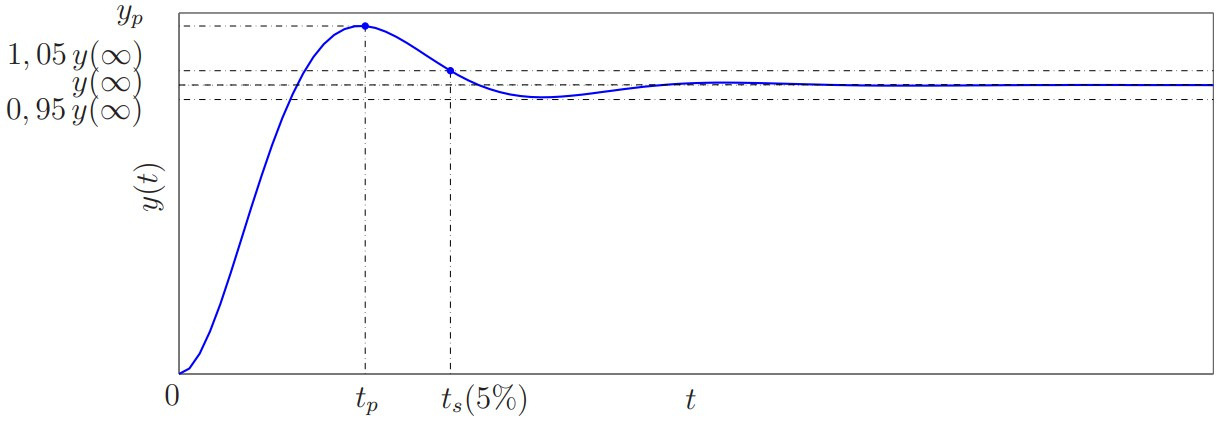
\includegraphics{Imagens/Lab3/Explicação/fig2.jpg}
\caption{Figura 2: Resposta de um sistema de segunda ordem sub-amortecido ao degrau.}
\end{figure}

Temos que
\[
y(\infty) = KA, \quad M_p= \frac {y_p-y(\infty)}{y(\infty)} = e^{\frac {-(\xi \pi)}{\sqrt{1-\xi^2}}}, \quad
t_p = \frac {\pi}{\omega_n\sqrt{1-\xi^2}}.
\]

Logo,

\begin{align}
K = \frac {y(\infty)}{A}, \quad M_p = \frac {y_p - y(\infty)}{y(\infty)}, \quad \xi = \sqrt{\frac {(\ln{M_p})^2}{(\ln{M_p})^2+\pi^2}}, \quad \omega_n = \frac {\pi}{t_p\sqrt{1-\xi^2}}.  \label{eq:eq34}
\end{align}

\hypertarget{sistemas-criticamente-amortecidos-e-super-amortecidos}{%
\subsubsection*{Sistemas criticamente amortecidos e super-amortecidos}\label{sistemas-criticamente-amortecidos-e-super-amortecidos}}
\addcontentsline{toc}{subsubsection}{Sistemas criticamente amortecidos e super-amortecidos}

Suponha que \(G(s)\) é estável com \(\xi \geq 1\) (criticamente amortecido ou super-amortecido). Neste caso, os dois pólos de \(G(s)\) são reais e a resposta ao degrau se assemelha ao de um sistema de primeira ordem (não apresenta oscilação nem sobressinal). Podemos identificar \(G(s)\) indiretamente através da identificação da Função de Transferência \(F(s)\) em malha-fechada. Considere o diagrama de blocos em malha-fechada mostrando na Figura 3, onde \(K_c > 0\) é o ganho de um controlador proporcional e \(r\) é a referência.

\begin{figure}
\centering
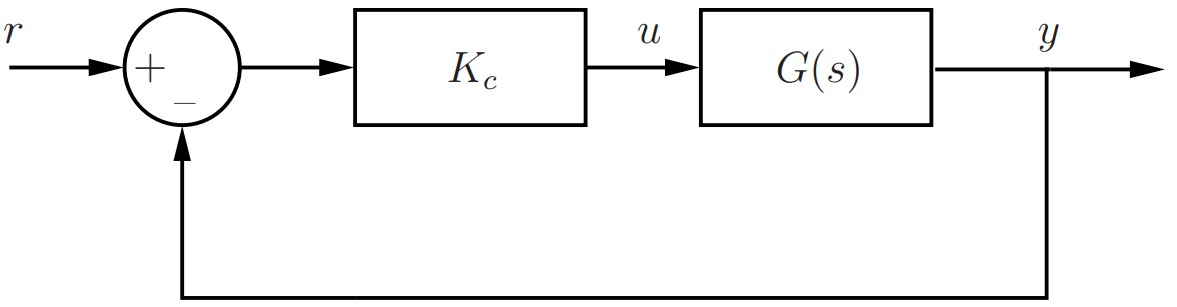
\includegraphics{Imagens/Lab3/Explicação/fig3.jpg}
\caption{Figura 3: Diagrama de blocos em malha-fechada.}
\end{figure}

Relembre que
\[
F(s) = \frac {Y(s)}{R(s)} = \frac {K_cG(s)}{1+K_cG(s)}.
\]

Para qualquer \(K_c > 0\), temos que \(F(s)\) é um sistema de segunda ordem estável. E, quando \(K_c > 0\) for suficientemente grade, temos que \(F(s)\) será um sistema de segunda ordem sub-amortecido. Assim, escolhemos \(K_c\) de modo que \(F(s)\) seja sub-amortecido e então identificamos \(F(s)\) conforme descrito na seção anterior aplicando uma referência \(r(t) = A\) do tipo degrau de magnitude \(A\). Desta maneira, identificaremos \(G(s)\) indiretamente pois

\begin{align}
F(s) = \frac {K_cG(s)}{1+K_cG(s)} \implies G(s) = \frac {F(s)}{K_c - K_cF(s)}.  \label{eq:eq35}
\end{align}

\hypertarget{problemas-laboratuxf3rio-3}{%
\chapter*{Problemas Laboratório 3}\label{problemas-laboratuxf3rio-3}}
\addcontentsline{toc}{chapter}{Problemas Laboratório 3}

Estes problemas são relacionados ao assunto abordado no Laboratório \ref{lab3}.

\hypertarget{problema-3.1}{%
\section*{Problema 3.1}\label{problema-3.1}}
\addcontentsline{toc}{section}{Problema 3.1}

Aplique um degrau \(u(t) = 2\) no Sistema 1 do arquivo \texttt{MatLab3.mdl} do Simulink. Pelas características da resposta, modele o Sistema 1 como uma Função de Transferência \(G_1(s)%
\) de primeira ou segunda ordem. Em seguida, identifique os parâmetros do modelo utilizando a equação \eqref{eq:eq32} ou \eqref{eq:eq34}. Compare a resposta do modelo identificado com a do Sistema 1.

\hypertarget{resoluuxe7uxe3o}{%
\subsubsection*{Resolução}\label{resoluuxe7uxe3o}}
\addcontentsline{toc}{subsubsection}{Resolução}

Simulando o sistema do modelo 1 obtemos o resultado abaixo.

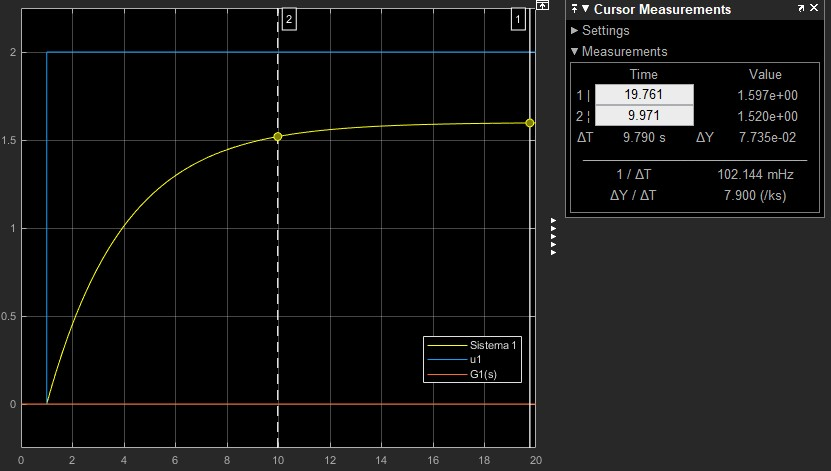
\includegraphics{Imagens/Lab3/Resolução/prob1A.jpg}

Pela curva feita espera-se que a Função de Transferência seja de primeira ordem. Utilizando as ferramentas fornecidas pelo \texttt{Simulink} foi estimado que
\[
y(\infty) = 1.6 \\ 
0.95y(\infty) = 1.52 \implies  t_s(5\%) = 9.97s \implies \tau = 3.33
\]

Assim,
\[
G_1(s) = \frac {0.8}{3.33s+1}.
\]

Simulando \(G_1(s)\), temos o resultado apresentado abaixo.

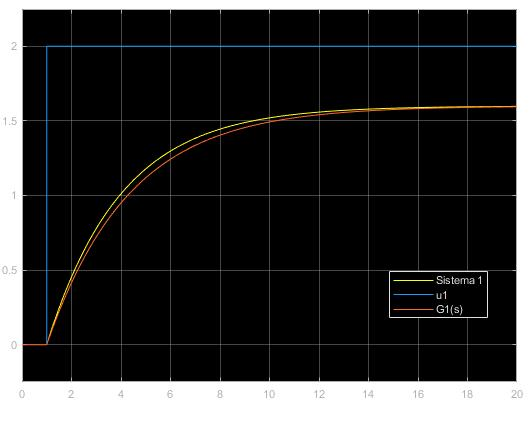
\includegraphics{Imagens/Lab3/Resolução/prob1B.jpg}

Percebe-se, assim, que a Função de Transferência \(G_1(s)\) se aproxima satisfatoriamente bem do Sistema 1.

\hypertarget{problema-3.2}{%
\section*{Problema 3.2}\label{problema-3.2}}
\addcontentsline{toc}{section}{Problema 3.2}

Aplique um degrau \(u(t) = 4\) no Sistema 2. Pelas características da resposta modele o Sistema 2 como uma Função de Transferência \(G_2(s)\) de primeira ou segunda ordem. Em seguida, identifique os parâmetros do modelo utilizando a equação \eqref{eq:eq32} ou \eqref{eq:eq34}. Realize os cálculos na linha de comando do \texttt{Matlab} (\(\ln{(x)} \implies \log{(x)}\) e \(\sqrt{x} \implies \text{sqrt(x)}\)).Compare a resposta do modelo identificando com a do Sistema 2.

\hypertarget{resoluuxe7uxe3o-1}{%
\subsubsection*{Resolução}\label{resoluuxe7uxe3o-1}}
\addcontentsline{toc}{subsubsection}{Resolução}

Simulando o sistema do modelo 1 obtemos o resultado abaixo.

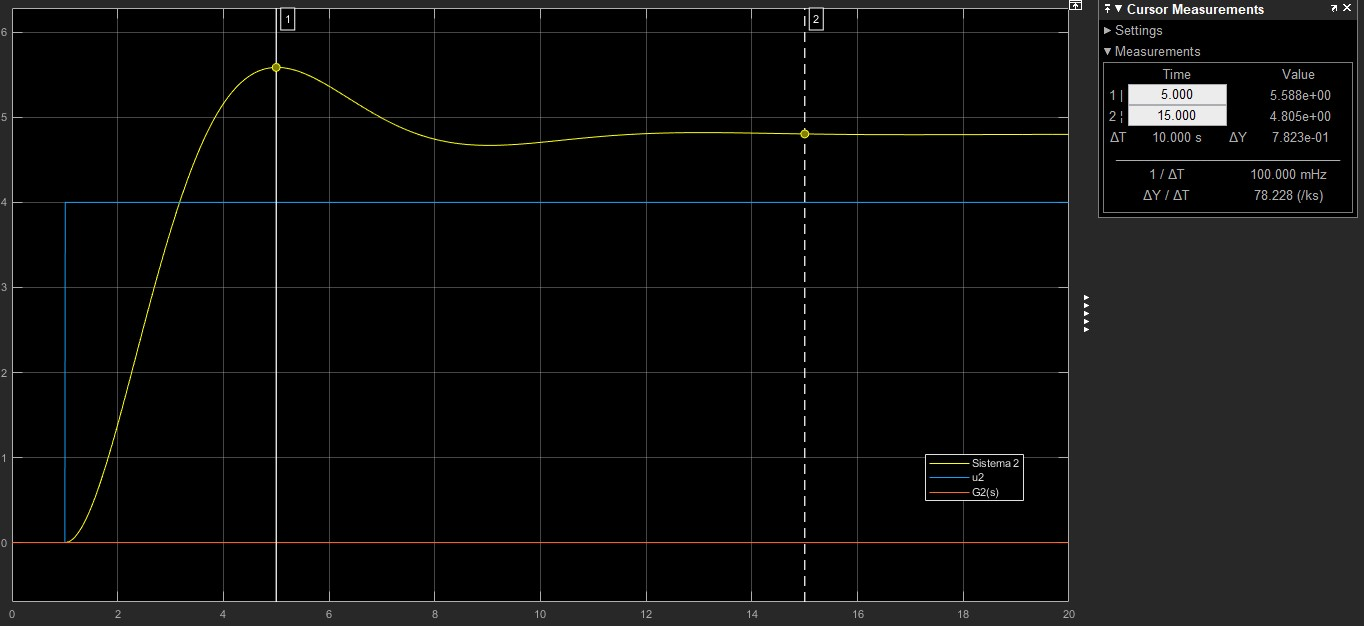
\includegraphics{Imagens/Lab3/Resolução/prob2A.jpg}

Pela curva feita espera-se que a Função de Transferência seja de segunda ordem. Utilizando as ferramentas fornecidas pelo \texttt{Simulink} foi estimado que
\[
y_p = 5.588 \\  
y(\infty) = 4.805 \\  
t_p = 5s
\]

Dessa forma, aplicando as equações 3.4, temos que
\[
K = 1.2, \quad M_p = 0.163, \quad \xi = 0.5 \quad \text{e} \quad \omega_n = 0.7255.
\]

Dessa forma, a Função de Transferência \(G_2(s)\) será
\[
G_2(s) = \frac {0.6316}{s^2 + 0.7255s + 0.5264}.
\]
Simulando \(G_2(s)\), temos o resultado apresentado abaixo.

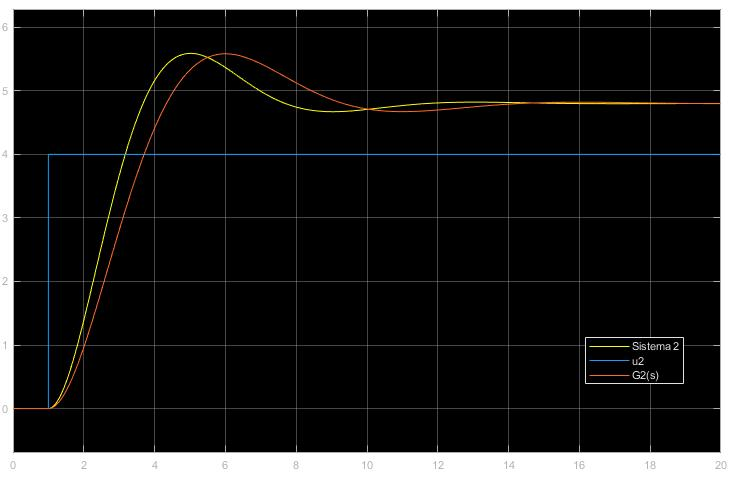
\includegraphics{Imagens/Lab3/Resolução/prob2B.jpg}

Percebe-se, assim, que a Função de Transferência \(G_2(s)\) se assemelha ao Sistema 2,porém, com menor precisão que a função \(G_1(s)\) se aproximou do Sistema 2.

\hypertarget{problema-3.3}{%
\section*{Problema 3.3}\label{problema-3.3}}
\addcontentsline{toc}{section}{Problema 3.3}

\hypertarget{parte-a}{%
\subsubsection*{Parte A}\label{parte-a}}
\addcontentsline{toc}{subsubsection}{Parte A}

Aplique um degrau \(u(t) = 3\) no Sistema 3. Obtenha um modelo aproximado para o Sistema 3 como uma Função de Transferência \(G(s)\) de primeira ordem. Agora implemente o diagrama de blocos em malha fechada da Figura 3 para o Sistema 3 com \(r(t) = 1\) do tipo degrau e \(K_c = 3\)Observamos que, na Figura 3, se \(G(s)\) é de primeira ordem, então a Função de Transferência em malha fechada \(F(s)\) também será de primeira ordem para qualquer valor de \(K_c > 0\). A resposta do Sistema 3 em malha-fechada está de acordo com tal propriedade? O que pode estar errado?

\hypertarget{resoluuxe7uxe3o-2}{%
\paragraph*{Resolução}\label{resoluuxe7uxe3o-2}}
\addcontentsline{toc}{paragraph}{Resolução}

Simulando o sistema do modelo 1 obtemos o resultado abaixo.

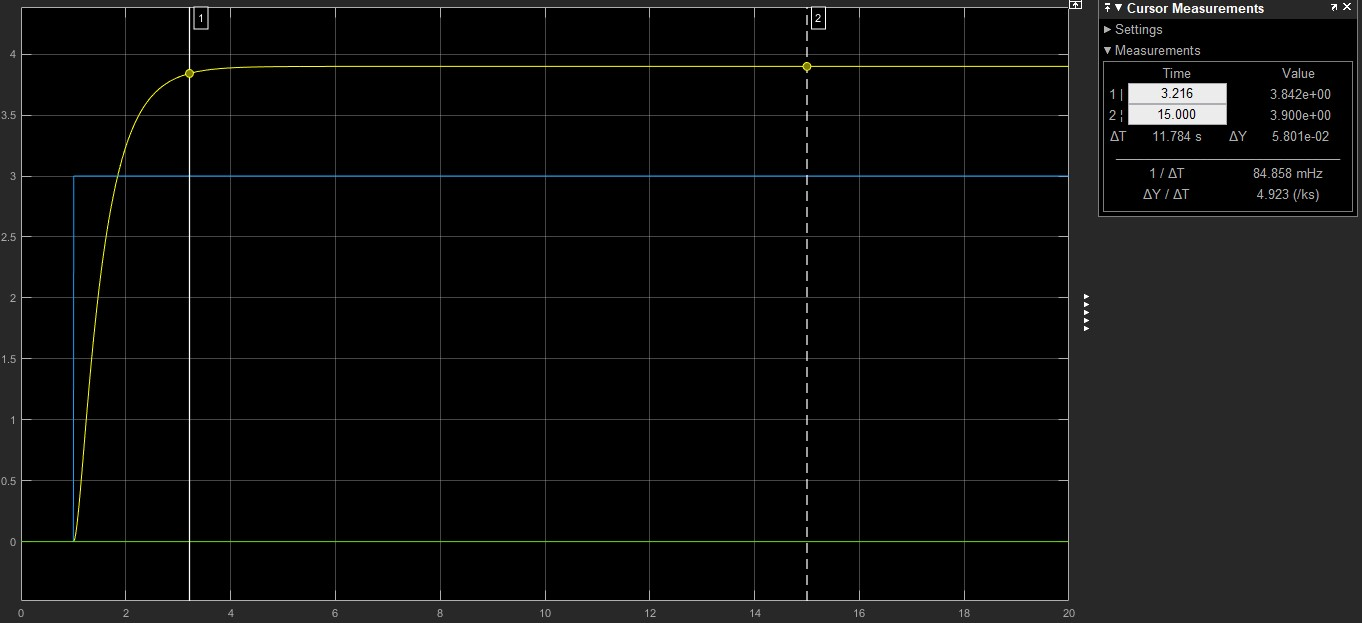
\includegraphics{Imagens/Lab3/Resolução/prob3AA.jpg}

Pela curva feita espera-se que a Função de Transferência seja de primeira ordem. Utilizando as ferramentas fornecidas pelo \texttt{Simulink} foi estimado que
\[
y(\infty) = 3.9 \\ 
0.95y(\infty) = 3.8415 \implies  t_s(5\%) = 3.22s \implies \tau = 1.072
\]

Assim,
\[
G_3(s) = \frac {1.3}{1.072s+1}.
\]

Simulando \(G_1(s)\), temos o resultado apresentado abaixo.

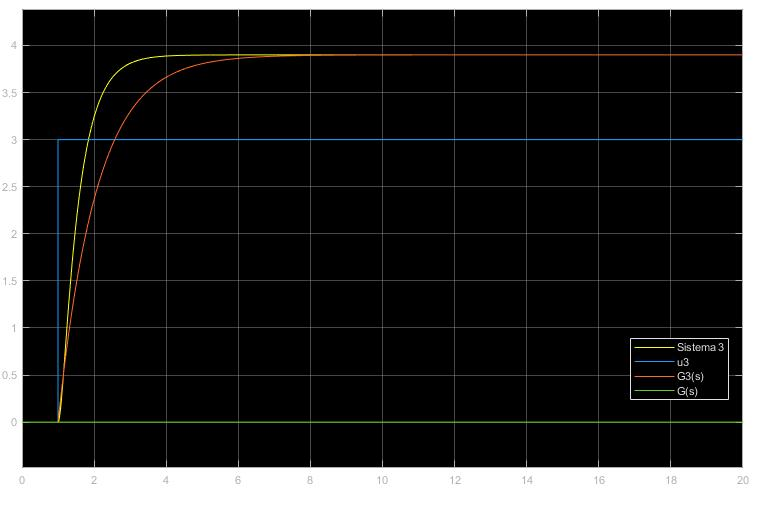
\includegraphics{Imagens/Lab3/Resolução/prob3AB.jpg}

Percebe-se, assim, que a Função de Transferência \(G_B(s)\) não se aproxima satisfatoriamente bem ao Sistema 3. Aplicando a malha fechada vista na figura 3, temos o resultado apresentado abaixo.

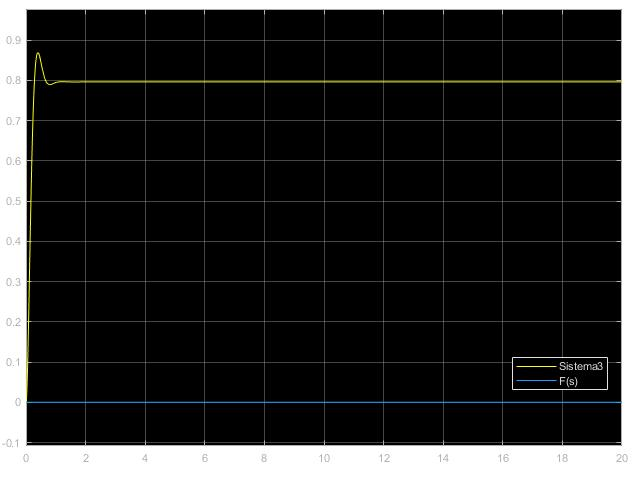
\includegraphics{Imagens/Lab3/Resolução/prob3AC.jpg}

Como \(K_c = 3 > 0\) e a Função de Transferência em malha fechada retornou um sistema de segunda ordem, percebe-se a resposta não está de acordo com a propriedade estabelecida. Desta forma, presume-se que \(G(s)\) não é de primeira ordem e sim de segunda.

\hypertarget{parte-b}{%
\subsubsection*{Parte B}\label{parte-b}}
\addcontentsline{toc}{subsubsection}{Parte B}

Identifique \(F(s)\). Em seguida, identifique \(G(s)\)indiretamente através da equação \eqref{eq:eq55}. Para isto, utilize os seguintes comandos no \texttt{Matlab}:

\begin{Shaded}
\begin{Highlighting}[]
\VariableTok{F} \OperatorTok{=} \VariableTok{tf}\NormalTok{([}\VariableTok{K}\OperatorTok{*}\VariableTok{wn}\OperatorTok{\^{}}\FloatTok{2}\NormalTok{]}\OperatorTok{,}\NormalTok{ [}\FloatTok{1} \FloatTok{2}\OperatorTok{*}\VariableTok{ksi}\OperatorTok{*}\VariableTok{wn} \VariableTok{wn}\OperatorTok{\^{}}\FloatTok{2}\NormalTok{])}
\VariableTok{G} \OperatorTok{=} \VariableTok{F}\OperatorTok{/}\NormalTok{(}\VariableTok{Kc}\OperatorTok{{-}}\VariableTok{Kc}\OperatorTok{*}\VariableTok{F}\NormalTok{)}
\VariableTok{G} \OperatorTok{=} \VariableTok{zpk}\NormalTok{(}\VariableTok{minreal}\NormalTok{(}\VariableTok{G}\NormalTok{)) }\CommentTok{\% minreal simplifica e zpk fatora}
\end{Highlighting}
\end{Shaded}

Note que \(G(s)\) é de segunda ordem com pólos reais. Neste momento, temos condições de responderm o que estava errado em nossa modelagem inicial do Sistema 3 como um sistema de primeira ordem. Compare a resposta em malha-aberta de \(G(s)\) (identificando indiretamente) com a do Sistema 3 para \(u(t) = 3\) do tipo degrau.

\hypertarget{resoluuxe7uxe3o-3}{%
\paragraph*{Resolução}\label{resoluuxe7uxe3o-3}}
\addcontentsline{toc}{paragraph}{Resolução}

Simulando o sistema do Sistema 3 em malha fechada e utilizando as ferramentas fornecidas pelo \texttt{Simulink} foi estimado que
\[
y_p = 0.868 \\ 
y(\infty) = 0.796 \\ 
t_p = 0.4s
\]

Assim, tem-se que:
\[
K = 0.796, \quad M_p = 0.09, \quad \xi = 0.61 \quad \text{e} \quad \omega_n= 9.888.
\]

Dessa forma, tem-se que
\[
F(s) = \frac {77.83}{s^2+ 12.01s +97.77}
\]
que gera a curva abaixo.

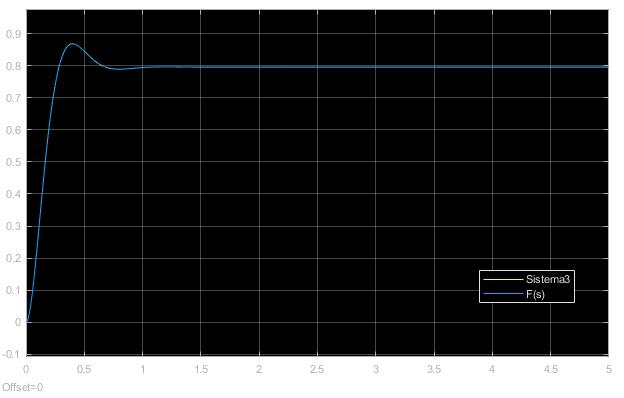
\includegraphics{Imagens/Lab3/Resolução/prob3BA.jpg}

Assim, é possível calcular \(G(s)\) a partir de \(F(s)\), tendo como resultado
\[
G(s) = \frac {25.94}{s^2+12.025s+19.96}.
\]

Agora é possível comprar \(G(s)\) com sua curva anterior, gerando o resultado abaixo.

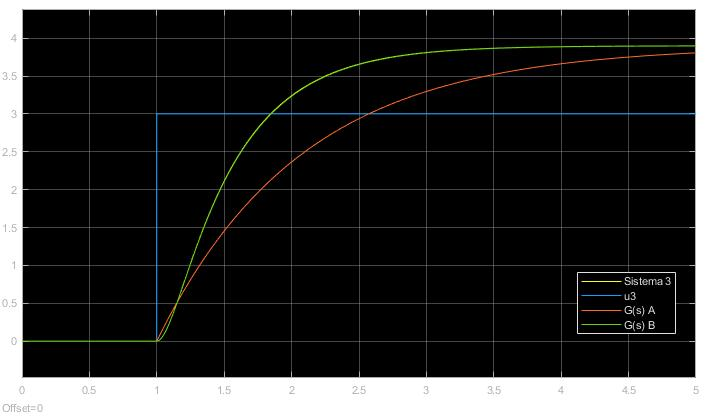
\includegraphics{Imagens/Lab3/Resolução/prob3BB.jpg}

Percebe-se que, considerando o modelo como uma Função de Transferência de segundo grau obtida através de \(F(s)\) é possível encontrar a curva exata correspondente ao Sistema 3.

\hypertarget{lab4}{%
\chapter{Rastreamento de Referências e Rejeição de Perturbações - Erro em Regime Permanente}\label{lab4}}

Nesta experiência analisaremos o erro em regime permanente de sistemas em malha-fechada para o rastreamento de referências e a rejeição de perturbações. Consideraremos referências e perturbações do tipo degrau, rampa e parábola. Comprovaremos os resultados teóricos através de simulações no Simulink/Matlab.

\hypertarget{tipos-de-sistemas}{%
\section{Tipos de Sistemas}\label{tipos-de-sistemas}}

Considere a Função de Transferência
\[
G(s) = \frac {N(s)}{D(s)}
\]
onde \(N(s)\) e \(D(s)\) são polinômios em \(s\) sem raízes em comum e com \(\text{grau}(N) \leq \text{grau}(D)\). Temos a seguinte classificação para \(G(s)\):

\begin{itemize}
\tightlist
\item
  Tipo 0: \(G(s)\) não possui pólos em \(s=0\). Denominamos \(K_p = G(0)\) de \emph{constante de posição}. Note que \(K_p = \lim\limits_{s \to 0} G(s)\).
\item
  Tipo 1: \(G(s)\) tem um (e apenas um) pólo em \(s=0\). Podemos então escrever \[G(s) = \frac {1}{s}G_0(s),\] onde \(G_0(s) = \frac {N(s)}{D_0(s)}\) não possui pólos em \(s=0\). Chamamos \(K_v= G_0(0) \neq 0\) de \emph{constante de velocidade}. Note que \(K_v = \lim\limits_{s \to 0} sG(s)\).
\item
  Tipo 2: \(G(s)\) tem dois (e apenas dois) pólos em \(s=0\). Podemos escrever \[G(s) = \frac {1}{s^2}G_0(s),\] onde \(G_0(s) = \frac {N(s)}{D_0(s)}\) não possui pólos em \(s=0\). Denominamos \(K_a = G_0(0) \neq 0\) de \emph{constante de aceleração}. Note que \(K_a =\lim\limits_{s \to 0} s^2G(s)\).
\end{itemize}

\hypertarget{erro-em-regime-permanente.}{%
\section{Erro em regime permanente.}\label{erro-em-regime-permanente.}}

Considere o sistema em malha-fechada com realimentação unitária mostrado na Figura @ref\{fig:fig41\}, onde:
\[
\begin{cases}
  y(t) & \quad \text{: saída}\\
  r(t) & \quad \text{: referência}\\
  e(t) = r(t)-y(t) & \quad \text{: erro de rastreamento}\\
  w(t) &\quad \text{: perturbação externa que não é possível de ser medida}
\end{cases}
\]

\begin{figure}
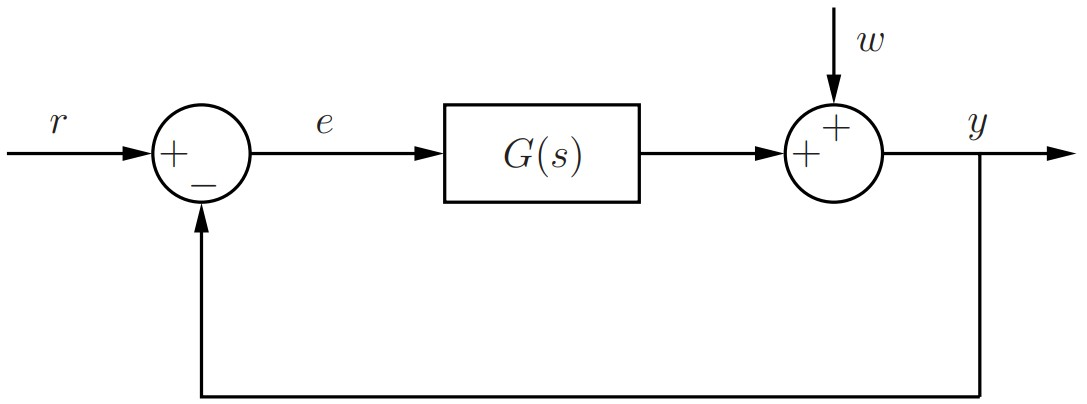
\includegraphics[width=0.8\linewidth]{Imagens/Lab4/Apresentação/fig1} \caption{Sistema em malha-fechada com perturbação na saída.}\label{fig:fig41}
\end{figure}

Desejamos analisar o erro em regime permanente (\(t \to \infty\)) quando existem perturbações externas. Temos que

\[
E(s) = R(s) - Y(s) = R(s) - [G(s)E(s) + W(s)]\\
\implies E(s) = \frac {1}{1 + G(s)}R(s) - \frac {1}{1+G(s)}W(s) \\
\implies E(s) = \underbrace{\frac {D(s)}{D(s) + N(s)}R(s)}_{E_R(s)} - \underbrace{\frac {D(s)}{D(s) + N(s)}W(s)}_{Y_W(s)}
\]

Note que \(E = E_R\) quando \(W= 0\) e que \(Y = Y_W\) quando \(R=0\). Podemos então analisar \(E\) através de \(E_R\) e \(Y_R\). O erro em regime permanente é dado por

\begin{align}
e(\infty) = \lim\limits_{t \to \infty}{e(t)} = e_r(\infty) - y_w(\infty), \label{eq:eq41}
\end{align}

desde que os limites \(e_r(\infty) = \lim\limits_{t\to \infty}{e_r(t)}\) e \(y_w(\infty) = \lim\limits_{t \to \infty}{y_w(t)}\) existam. Dizemos que há \emph{rastreamento de referência} quando \(e_r(\infty) = 0\). De maneira semelhante, dizemos que há \emph{rejeição de perturbação} quando \(y_w(\infty) = 0\). Portanto, quando há rastreamento de referência e rejeição de perturbação teremos que \(e(\infty) = 0\).

Iremos agora analisar \(e_r(\infty)\) e \(y_w(\infty)\) através de \(E_R(s)\) e \(Y_W(s)\), respectivamente, considerando que a referência \(r\) e a perturbação externa \(w\) são do tipo degrau, rampa ou parábola. Relembramos que:

\begin{enumerate}
\def\labelenumi{\arabic{enumi}.}
\tightlist
\item
  Degrau: \(x(t) = A \iff X(s) = \frac {A}{s}\)
\item
  Rampa: \(x(t) = Bt \iff X(s) = \frac {B}{s^2}\)
\item
  Parábola: \(x(t) = Ct^2 \iff X(s) = \frac {2C}{s^3}\)
\end{enumerate}

Suponha que \(D(s) + N(s) = 0\) possui todas as raízes no SPE (Semi-Plano Esquerdo do plano \(s\)) e que \(D(s)R(s)\) e \(D(s)W(s)\) possuem no máximo um pólo em \(s=0\). Isto garante que \(e_r(\infty)\) e \(y_w(\infty)\) existem e, assim, o Teorema do Valor Final pode ser aplicado. Ressaltamos que as raízes de \(D(s) + N(s) = 0\) nada mais são do que os pólos da Função de Transferência de malha-fechada quando não há perturbação (\(w=0\))
\[
F(s) = \frac {Y(s)}{R(s)} = \frac{G(s)}{1+G(s)} = \frac {N(s)}{D(s)+N(s)}, \quad \text{(para } w=0 \text{).} 
\]

Desse modo, estamos assumindo que \(F(s)\) é estável para \(w=0\). Com base no Teorema do Valor Final, podemos construir a tabela \ref{tab:tab41} e a tabela \ref{tab:tab42} mostradas abaixo. Note que os valores de \(e_r(\infty)\) e de \(y_w(\infty)\) (regime permanente) dependem apenas da constante de posição \(K_p\), da constante de velocidade \(K_v\) e da cosntante de aceleração \(K_a\). Tl nomenclatura tem origem em sistemas mecânicos de controle. Por exemplo, para um sistema Tipo 0 e \(r(t)=A\) (degrau) temos que (Teorema do Valor Final)
\[
e_r(\infty) = \lim\limits_{s \to 0}{sE_R(s)}=\lim\limits_{s\to0}{\frac{D(s)}{D(s)+N(s)}\frac{A}{s}} = \lim\limits_{s\to0}{\frac{AD(s)}{D(s)+N(s)}} \\
= \frac{AD(0)}{D(0) + N(0)} = \frac{A}{1+N(0)/D(0)} = \frac{A}{1+G(0)} = \frac {A}{1+K_p}.
\]
pois como \(D(0) + N(0) \neq 0\) (\(F(s)\) é estável) e \(D(0) \neq 0\) (\(G(0)\) é de Tipo 0) não há divisão por zero!

E, para um sistema Tipo 2 e \(r(t) = Bt\) (rampa), temos \(G(s) = \frac{N(s)}{D(s)} = \frac{N(s)}{s^2D_0(s)}\) e
\[
e_r(\infty) = \lim\limits_{s \to 0}{sE_r(s) = \lim\limits_{s \to 0}{s\frac{D(s)}{D(s)+N(s)}\frac{B}{s^2}}} = \lim\limits_{s \to 0}{s\frac{s^2D_0(s)}{D(s)+N(s)}\frac{B}{s^2}}\\
=\lim\limits_{s \to 0}{\frac{sBD_0(s)}{D(s)+N(s)}}=\frac{0BD(0)}{N(0)+D(0)}=0,
\]
pois \(D(0) + N(0) \neq 0\) (\(F(s)\) é estável) e não há divisão por zero!

Observamos que a tabela \ref{tab:tab41} e a tabela \ref{tab:tab42} são válidas apenas para sistemas com realimentação unitária com perturbação na saída (veja a Figura \ref{fig:fig41}) e tais que a Função de Transferência em malha-fechada é estável para \(w=0\).

\begin{table}

\caption{\label{tab:tab41}Valores de $e_r(\infty)$ ($w=0$)}
\centering
\begin{tabular}[t]{llll}
\toprule
Sistema $G(s)$ / Referência & $r(t)=A$ & $r(t) = Bt$ & $r(t) = Ct^2$\\
\midrule
Tipo 0 & $\frac{A}{1 + K_p}$ & $\infty$ & $\infty$\\
Tipo 1 & 0 & $\frac{B}{K_v}$ & $\infty$\\
Tipo 2 & 0 & 0 & $\frac{2C}{K_a}$\\
\bottomrule
\end{tabular}
\end{table}

\begin{table}

\caption{\label{tab:tab42}Valores de $y_r(\infty)$ ($r=0$ e $w$ na saída de $G(s)$)}
\centering
\begin{tabular}[t]{llll}
\toprule
Sistema $G(s)$ / Perturbação & $w(t)=A$ & $w(t) = Bt$ & $w(t) = Ct^2$\\
\midrule
Tipo 0 & $\frac{A}{1 + K_p}$ & $\infty$ & $\infty$\\
Tipo 1 & 0 & $\frac{B}{K_v}$ & $\infty$\\
Tipo 2 & 0 & 0 & $\frac{2C}{K_a}$\\
\bottomrule
\end{tabular}
\end{table}

Agora, considere o sistema mostrado na Figura \ref{fig:fig42} e assuma que \(G_2(s)\) não possui \emph{zeros} em \(s=0\). Para tal sistema, a Tabela \ref{tab:tab41} continua válida para \(G(s) = G_1(s)G_2(s)\). No entanto, a Tabela \ref{tab:tab42} deve ser substituída pela Tabela \ref{tab:tab43}. Ressaltamos que os valores \(\neq 0\) na Tabela \ref{tab:tab43} podem ser calculados analiticamente a partir de \(G_1(s) \text{ e } G_2(s)\). Entretanto, isso não é o objeto de estudo desta experiência.

\begin{figure}
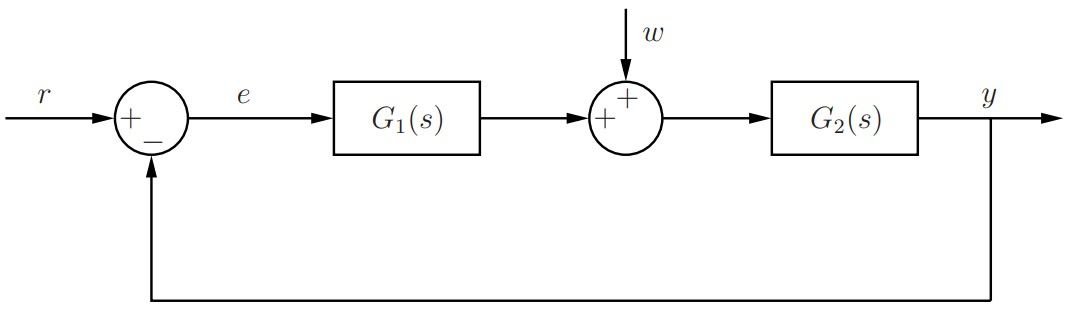
\includegraphics[width=0.8\linewidth]{Imagens/Lab4/Apresentação/fig2} \caption{Sistema em malha-fechada com perturbação na entrada de $G_s(s)$ e $G_2(s)$ não possui *zeros* em $s=0$.}\label{fig:fig42}
\end{figure}

\begin{table}

\caption{\label{tab:tab43}Valores de $y_r(\infty)$ ($r=0$ e $w$ na saída de $G_2(s)$)}
\centering
\begin{tabular}[t]{llll}
\toprule
Sistema $G(s)$ / Perturbação & $w(t)=A$ & $w(t) = Bt$ & $w(t) = Ct^2$\\
\midrule
Tipo 0 & $\neq 0$ & $\infty$ & $\infty$\\
Tipo 1 & 0 & $\neq 0$ & $\infty$\\
Tipo 2 & 0 & 0 & $\neq 0$\\
\bottomrule
\end{tabular}
\end{table}

\hypertarget{problemas-laboratuxf3rio-4}{%
\chapter*{Problemas Laboratório 4}\label{problemas-laboratuxf3rio-4}}
\addcontentsline{toc}{chapter}{Problemas Laboratório 4}

Estes problemas são relacionados ao assunto abordado no Laboratório \ref{lab4}.

Em todos os itens abaixo consideramos o sistema em malha-fechada mostrado na Figura \ref{fig:fig43} onde \(C(s)\) é o controlador, \(G(s)\) é a planta (processo) e \(u(t)\) é o sinal de controle.

\begin{figure}
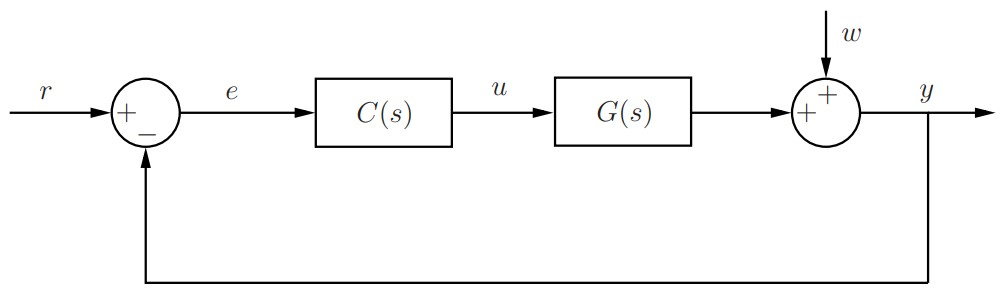
\includegraphics[width=0.8\linewidth]{Imagens/Lab4/Apresentação/fig3} \caption{Sistema em malha-fechada.}\label{fig:fig43}
\end{figure}

\hypertarget{problema-4.1}{%
\section*{Problema 4.1}\label{problema-4.1}}
\addcontentsline{toc}{section}{Problema 4.1}

Considere que

\[
G(s) = \frac {1}{0.5s+1}, \quad C(s) = K_c \quad \text{(proporcional)}, \quad w=0 \quad \text{(sem perturbação)}.
\]

\begin{enumerate}
\def\labelenumi{\alph{enumi}.}
\tightlist
\item
  Simule para \(r(t) = 1\) (degrau unitário) e \(K_c = 1\) Determine \(e(\infty) = e_r(\infty)\) por simulação e compare com a Tabela \ref{tab:tab41} (note que \(K_p = Kc\)). Repita para \(K_c = 10\) e \(K_c = 100\), analisando também o regime transitório de saída \(y(t)\).
\item
  Percebemos que \(e(\infty)\) diminui a medida que aumentamos o ganho \(K_c\) do controlador. Poderíamos então escolher \(K_c = \infty\) para que \(e(\infty) = 0\)? Justifique sua resposta (dica: observe o sinal de controle \(u(t)\)).
\item
  Com \(K_c = 1\) simule para \(r(t) = t\) (rampa) e \(r(t) = 0.5t^2\) (parábola). Determine o erro em regime permanente e verifique se os resultados estão de acordo com o esperado.
\end{enumerate}

\hypertarget{resoluuxe7uxe3o}{%
\subsubsection*{Resolução}\label{resoluuxe7uxe3o}}
\addcontentsline{toc}{subsubsection}{Resolução}

\hypertarget{parte-a}{%
\subsubsection*{Parte A}\label{parte-a}}
\addcontentsline{toc}{subsubsection}{Parte A}

Por meio da simulação foi encontrado o valor de \(e(\infty) = e_r(\infty) = 0.5\) conforme apresenta a Figura \ref{fig:fig41A1}.

\begin{figure}
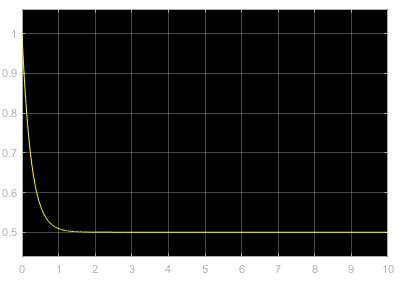
\includegraphics[width=0.8\linewidth]{Imagens/Lab4/Resolução/prob1A1} \caption{Valor de $e(r)$.}\label{fig:fig41A1}
\end{figure}

Utilizando a Tabela \ref{tab:tab41} temos que \(e_r(\infty)=\frac{A}{1 + K_p}\). Assim, tendo \(A = 1\) e \(K_c = 1\), temos que \(e_r(\infty) = \frac {1}{2} = 0.5\), o que está de acordo com o resultado encontrado na simulação. A figura \ref{fig:fig41A2} apresenta os valores de \(e(s) = e_r(s)\) e \(Y(s)\) para \(K_c = 10\) e \(K_c = 100\).

\begin{figure}
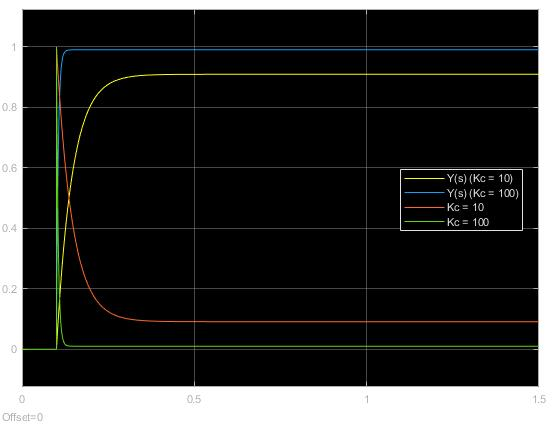
\includegraphics[width=0.8\linewidth]{Imagens/Lab4/Resolução/prob1A2} \caption{Valores para $K_c = 10$ e $K_c = 100$.}\label{fig:fig41A2}
\end{figure}

\hypertarget{parte-b}{%
\subsubsection*{Parte B}\label{parte-b}}
\addcontentsline{toc}{subsubsection}{Parte B}

Teoricamente, é possível encontrar um erro nulo \(e(\infty) = 0\) se utilizado um ganho infinito \(K_c = \infty\). Pois, de acordo com a Tabela \ref{tab:tab41}, temos que
\[
e(\infty) = \frac {A}{1+K_c} = \frac {A}{1+\infty} = 0.
\]

Entretanto, não existe um sistema prático que retorne um ganho infinito. O ideal seria considerar um sistema que seja de Tipo 1 ou 2 para que, ao aplicar uma entrada do tipo degrau ele retorne um erro nulo.

\hypertarget{parte-c}{%
\subsubsection*{Parte C}\label{parte-c}}
\addcontentsline{toc}{subsubsection}{Parte C}

A Figura \ref{fig:fig41C1} apresenta os valores de \(y(s)\) e \(e(s)\) para uma entrada \(r(t) = t\) (rampa).

\begin{figure}
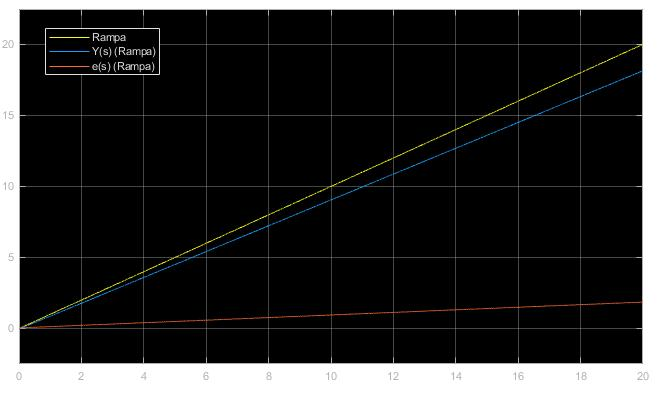
\includegraphics[width=0.8\linewidth]{Imagens/Lab4/Resolução/prob1C1} \caption{Valores para entrada do tipo rampa.}\label{fig:fig41C1}
\end{figure}

A Figura \ref{fig:fig41C2} apresenta os valores de \(y(s)\) e \(e(s)\) para uma entrada \(r(t) = 0.5t^2\) (parábola).

\begin{figure}
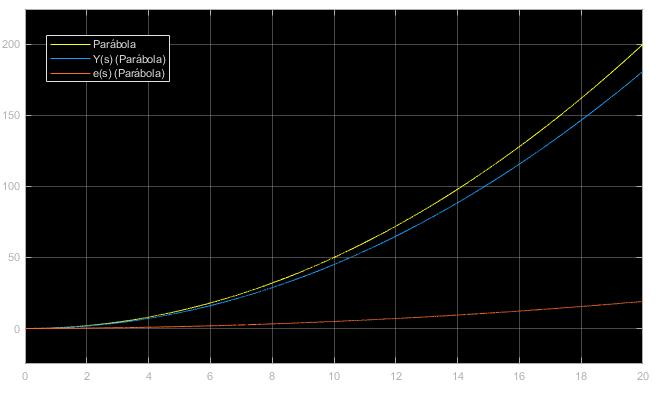
\includegraphics[width=0.8\linewidth]{Imagens/Lab4/Resolução/prob1C2} \caption{Valores para entrada do tipo parábola.}\label{fig:fig41C2}
\end{figure}

É possível perceber que, como o esperado, \(e(\infty)= e_r(\infty) = \infty\) para ambos os casos.

\hypertarget{problema-4.2}{%
\section*{Problema 4.2}\label{problema-4.2}}
\addcontentsline{toc}{section}{Problema 4.2}

Considere que
\[
G(s) = \frac {1}{0.5s+1}, \quad C(s) = \frac{K_c}{s} \text{ (integral)}, \quad w=0 \text{ (sem perturbação).}
\]

\begin{enumerate}
\def\labelenumi{\alph{enumi}.}
\tightlist
\item
  Simule para \(r(t) = 1\) (degrau unitário) e \(K_c = 1\). Determine \(e(\infty) = e_r(\infty)\) por simulação e compare com a Tabela \ref{tab:tab41}. Analise também o regime transitório da saída para \(y(t)\) (sobressinal, por exemplo). Repita para \(K_c = 10\). Observe o aumento no sobressinal.
\item
  Simule para \(K_c = 2\) e \(r(t) = t\) (rampa). Determine \(e(\infty)\) por simulação e compare com a Tabela \ref{tab:tab41} (note que \(K_v = K_c\)). Encontre analiticamente \(K_c\) de modo que o erro à rampa \(r(t) = t\) em regime permanente seja igual a 0.1. Agora verifique se as simulações estão de acordo com o valor calculado de \(K_c\).
\item
  Simule para \(K_c = 2\) e \(r(t) = 0.5t^2\) (parábola). Determine o erro em regime permanente por simulação e analise os resultados.
\item
  Agora suponha que
  \[
  G(s) = \frac {-s+2}{0.5s+1}, \quad C(s)= \frac{2}{s}, \quad r(t) = 1 \text{ (degrau).}
  \]
  Determine \(e(\infty)\) por simulação. Note que o erro não converge para zero. O resultado está de acordo com o esperado? Relembre que a Tabela \ref{tab:tab41} e a Tabela \ref{tab:tab42} são validas apenas quando o sistema em malha-fechada para \(w=0\) é estável (os pólos estão no SPE).
\end{enumerate}

\hypertarget{resuluuxe7uxe3o}{%
\subsubsection*{Resulução}\label{resuluuxe7uxe3o}}
\addcontentsline{toc}{subsubsection}{Resulução}

\hypertarget{parte-a-1}{%
\paragraph*{Parte A}\label{parte-a-1}}
\addcontentsline{toc}{paragraph}{Parte A}

Aplicando um controle \(C(s) = \frac {K_c}{s}\) em série a uma função \(G(s) = \frac {1}{0.5s+1}\) temos como resultado a Função de Transferência\\
\[
G_t(s) = C(s)G(s) = \frac {K_c}{s} \frac{1}{0.5s+1} = \frac {K_c}{s(0.5s+1)},
\]
que não possui zeros e possui pólos em \(s = 0\) e \(s = 2\). Deste modo, o sistema se caracteriza como um sistema do Tipo 1. Simulando o sistema temos como resultado a Figura \ref{fig:fig42A1}.

\begin{figure}
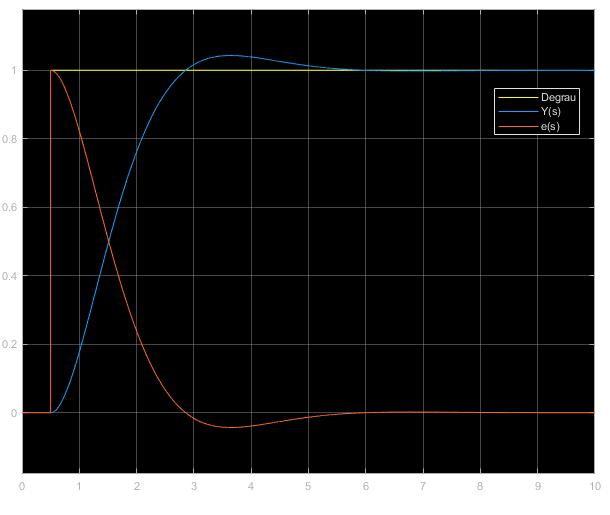
\includegraphics[width=0.8\linewidth]{Imagens/Lab4/Resolução/prob2A1} \caption{Valores para $K_c = 1$.}\label{fig:fig42A1}
\end{figure}

Simulando para \(K_c = 10\), temos o resultado abaixo.

\begin{figure}
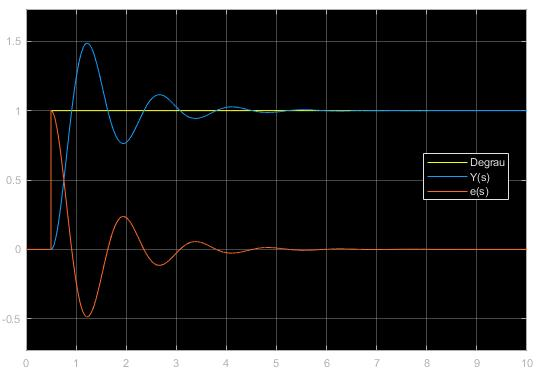
\includegraphics[width=0.8\linewidth]{Imagens/Lab4/Resolução/prob2A2} \caption{Valores para $K_c = 10$.}\label{fig:fig42A2}
\end{figure}

\hypertarget{parte-b-1}{%
\paragraph*{Parte B}\label{parte-b-1}}
\addcontentsline{toc}{paragraph}{Parte B}

Simulando o sistema para um \(K_c = 2\) e uma entrada tipo rampa, temos que o sistema tem \(e(\infty) = 0.5\), o que está de acordo com a Tabela \ref{tab:tab41}. O resultado da simulação está apresentado abaixo.

\begin{figure}
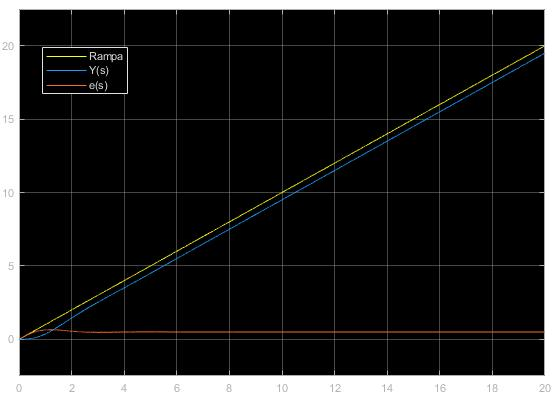
\includegraphics[width=0.8\linewidth]{Imagens/Lab4/Resolução/prob2B1} \caption{Valores para $K_c = 2$ e entrada do tipo rampa.}\label{fig:fig42B1}
\end{figure}

Analiticamente, é possível calcular o valor de \(K_v\) para que \(e(\infty) = 0.1\).

\[
0.1 = \frac {1}{K_v} \implies K_v = 10
\]

Simulando o sistema o valor foi comprovado.

\begin{figure}
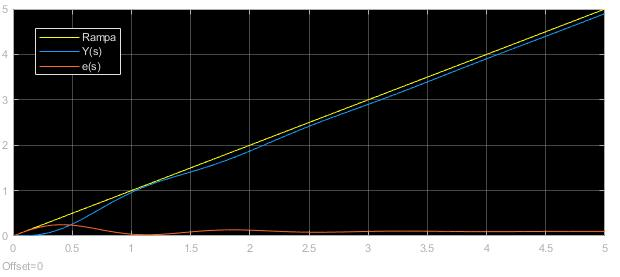
\includegraphics[width=0.8\linewidth]{Imagens/Lab4/Resolução/prob2B2} \caption{Valores para $K_c = 10$ e entrada do tipo rampa.}\label{fig:fig42B2}
\end{figure}

\hypertarget{parte-c-1}{%
\paragraph*{Parte C}\label{parte-c-1}}
\addcontentsline{toc}{paragraph}{Parte C}

Simulando o sistema para \(K_c = 2\) e uma entrada do tipo parábola, temos \(e(\infty) = \infty\), o que está de acordo com a Tabela \ref{tab:tab41}.

\begin{figure}
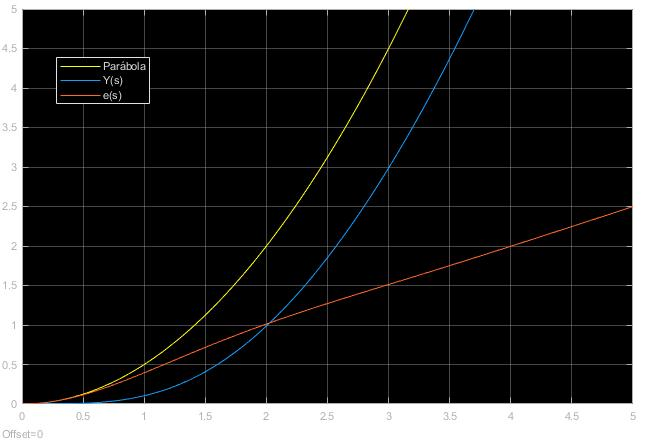
\includegraphics[width=0.8\linewidth]{Imagens/Lab4/Resolução/prob2C1} \caption{Valores para $K_c = 2$ e entrada do tipo parábola.}\label{fig:fig42C1}
\end{figure}

\hypertarget{parte-d}{%
\paragraph*{Parte D}\label{parte-d}}
\addcontentsline{toc}{paragraph}{Parte D}

Simulando a Função de Transferência \(G(s) = \frac {-s+2}{0.5s +1}\), controle \(C(s) = \frac {2}{s}\) e entrada do tipo degrau temos o resultado apresentado na Figura \ref{fig:fig42D1}.

\begin{figure}
\includegraphics[width=0.8\linewidth]{Imagens/Lab4/Resolução/prob2D1} \caption{Valores de $e(s)$ e $y(s)$.}\label{fig:fig42D1}
\end{figure}

Diferentemente do esperado (que o \(e(\infty) = 0\)) uma vez que segundo a Tabela \ref{tab:tab41} para sistemas do Tipo 1 para entrada igual degrau o erro esperado é nulo, o erro não converge. Na realidade, é possível notar que o sistema não se comportou de forma estável.

\hypertarget{problema-4.3}{%
\section*{Problema 4.3}\label{problema-4.3}}
\addcontentsline{toc}{section}{Problema 4.3}

Considere que
\[
G(s) = \frac {1}{0.5s +1}, \quad C(s) = \frac {2}{s} \text{ (integral)}.
\]

\begin{enumerate}
\def\labelenumi{\alph{enumi}.}
\tightlist
\item
  Determine \(y(\infty) = y(\infty)\) por simulação para \(w =1\) (degrau unitário) e \(r=0\). Compare com a Tabela \ref{tab:tab42}.
\item
  Considere que \(r(t) = 5\) (degrau em \(t=0\)) e aplique uma perturbação \(w=1\) (degrau) no instante \(t=9\). Determine \(e(\infty)\) e analise os resultados (talvez seja necessário aumentar o tempo de simulação).
\item
  Considere que \(r(t) = 2t\) (rampa) e \(w=0\). Determine \(e(\infty) = e_r(\infty)\) por simulação e compare com a Tabela \ref{tab:tab41}.
\item
  Considere que \(r(t) = 0\) e \(w=t\) (rampa). Determine \(y(\infty) = y_w(\infty)\) por simulação e compare com a Tabela \ref{tab:tab42}.
\item
  Considere que \(r(t) = 2t\) (rampa) e \(w=t\) (rampa). Determine \(e(\infty)\) por simulação e verifique que tal valor é a diferença dos valores obtidos nas letras c e d.~Tal resultado era esperado? Justifique (relembre \eqref{eq:eq41}).
\end{enumerate}

\hypertarget{resoluuxe7uxe3o-1}{%
\subsubsection*{Resolução}\label{resoluuxe7uxe3o-1}}
\addcontentsline{toc}{subsubsection}{Resolução}

\hypertarget{parte-a-2}{%
\paragraph*{Parte A}\label{parte-a-2}}
\addcontentsline{toc}{paragraph}{Parte A}

Simulando o sistema com uma referência em zero e uma perturbação do tipo degrau unitário, temos o resultado apresentando na Figura \ref{fig:fig43A1} que está de acordo com o resultado esperado da Tabela \ref{tab:tab42}, retornando um valor de \(y(\infty) = 0\)

\begin{figure}
\includegraphics[width=0.8\linewidth]{Imagens/Lab4/Resolução/prob3A1} \caption{Valores para sistema sem referência, apenas com perturbação.}\label{fig:fig43A1}
\end{figure}

\hypertarget{parte-b-2}{%
\paragraph*{Parte B}\label{parte-b-2}}
\addcontentsline{toc}{paragraph}{Parte B}

Simulando o sistema tendo uma entrada degrau de amplitude 5 e uma perturbação de amplitude 1, temos o resultado apresentado na figura \ref{fig:fig43B1}. O resultado mostra que o sistema era estável e havia convergido para 0. Ao receber a perturbação, o sistema se comportou de forma semelhante (a resposta voltou ao pico do sobressinal que havia chegado inicialmente) ao início da simulação, voltando a convergir para 0 em \(t=\infty\).

\begin{figure}
\includegraphics[width=0.8\linewidth]{Imagens/Lab4/Resolução/prob3B1} \caption{Valores para referência tipo degrau com perturbação.}\label{fig:fig43B1}
\end{figure}

\hypertarget{parte-c-2}{%
\paragraph*{Parte C}\label{parte-c-2}}
\addcontentsline{toc}{paragraph}{Parte C}

A simulação para um sistema com referência \(r(t) = 2t\) e sem perturbação é mostrada na Figura \ref{fig:fig43C1}.

\begin{figure}
\includegraphics[width=0.8\linewidth]{Imagens/Lab4/Resolução/prob3C1} \caption{Valores para rampa sem perturbação.}\label{fig:fig43C1}
\end{figure}

Percebe-se que o resultado está de acordo com o esperado, pois, de acordo com a tabela \ref{tab:tab41}, temos que
\[
e(\infty) = \frac {B}{K_v} = \frac {2}{2} = 1.
\]

\hypertarget{parte-d-1}{%
\paragraph*{Parte D}\label{parte-d-1}}
\addcontentsline{toc}{paragraph}{Parte D}

A simulação para um sistema com referência nula e perturbação \(w(t) = t\) é mostrada na Figura \ref{fig:fig43D1}.

\begin{figure}
\includegraphics[width=0.8\linewidth]{Imagens/Lab4/Resolução/prob3D1} \caption{Valores para rampa sem perturbação.}\label{fig:fig43D1}
\end{figure}

Percebe-se que o resultado está de acordo com o esperado, pois, de acordo com a tabela \ref{tab:tab42}, temos que
\[
y(\infty) = \frac {B}{K_v} = \frac {1}{2} = 0.5.
\]

\hypertarget{parte-e}{%
\paragraph*{Parte E}\label{parte-e}}
\addcontentsline{toc}{paragraph}{Parte E}

A simulação para um sistema com referência \(r(t) = 2t\) e perturbação \(w(t) = t\) é mostrada na Figura \ref{fig:fig43E1}.

\begin{figure}
\includegraphics[width=0.8\linewidth]{Imagens/Lab4/Resolução/prob3E1} \caption{Valores para referência e perturbação tipo rampa.}\label{fig:fig43E1}
\end{figure}

Percebe-se que o resultado está de acordo com o esperado, pois, de acordo com a equação \eqref{eq:eq41}, temos que
\[
e(\infty) = e_r(\infty) - y_w(\infty) = 1 - 0.5 = 0.5
\]

\hypertarget{problema-4.4}{%
\section*{Problema 4.4}\label{problema-4.4}}
\addcontentsline{toc}{section}{Problema 4.4}

Considere que
\[
G(s) = \frac {2s +1}{0.5s+1}, \quad C(s) = \frac {K_c}{s^2}, \quad r(t) = t, \quad w(t) = 0.1t.
\]

\begin{enumerate}
\def\labelenumi{\alph{enumi}.}
\tightlist
\item
  Considere que \(K_c =1\). Determine \(e(\infty)\) por simulação. O Resultado está de acordo com o esperado?
\item
  Considere que \(K_c =2\), \(r(t) = t^2\), \(w(t) = 0.5t^2\). Determine \(e(\infty)\) por simulação e verifique se o mesmo está de acordo com o esperado. Note que \(K_a = K_c\).
\end{enumerate}

\hypertarget{parte-a-3}{%
\subsubsection*{Parte A}\label{parte-a-3}}
\addcontentsline{toc}{subsubsection}{Parte A}

O resultado da simulação está apresentado na Figura \ref{fig:fig44A1}.

\begin{figure}
\includegraphics[width=0.8\linewidth]{Imagens/Lab4/Resolução/prob4A1} \caption{Valores para rampa com perturbação.}\label{fig:fig44A1}
\end{figure}

O resultado era esperado pois, para uma entrada tipo rampa com perturbação tipo rampa, um sistema do Tipo 2 retorna \(e_r(\infty) = 0\) e \(y_w(\infty) = 0\), resultando em \(e(\infty) = 0\).

\hypertarget{parte-b-3}{%
\subsubsection*{Parte B}\label{parte-b-3}}
\addcontentsline{toc}{subsubsection}{Parte B}

O resultado da simulação está apresentado na Figura \ref{fig:fig44B1}.

\begin{figure}
\includegraphics[width=0.8\linewidth]{Imagens/Lab4/Resolução/prob4B1} \caption{Valores para parábola com perturbação.}\label{fig:fig44B1}
\end{figure}

O resultado era esperado pois temos (\(e_r(\infty)\) e \(y_w(\infty)\) obtidos por meio de simulação)
\[
e_r(\infty) = 0.5 \\
y_w(\infty) = 0.25 \\
e(\infty) = 0.25.
\]

\hypertarget{lab5}{%
\chapter{Projeto de Controladores por Métodos Algébricos}\label{lab5}}

Nesta experiência projetaremos controladores que atendam determinadas especificações de regime transitório e de regime permanente em malha-fechada por métodos algébricos. Comprovaremos por simulação no Matlab o desempenho do sistema em malha-fechada.

\hypertarget{controladores-cluxe1ssicos}{%
\section{Controladores Clássicos}\label{controladores-cluxe1ssicos}}

Considere o diagrama de blocos \(G(s)\) em malha-fechada da Figura \ref{fig:fig51} onde \(r(t)\) é a referência, \(w(t)\) é uma perturbação externa, \(y(t)\) é a saída, \(e(t) = r(t) - y(t)\) é o erro de rastreamento, \(u(t)\) é o controle e \(C(s)\) é o controlador a ser projetado.

Relebramos que se \(G(s) = \frac {N(s)}{D(s)}\) então os \emph{zeros} de \(G(s)\) são as raízes de \(N(s)\) e os \emph{pólos} de \(G(s)\) são as raízes de \(D(s)\). Além disso, uma Função de Transferência é estável quando todos os pólos estão no SPE (Semi-Plano Esquerdo do plano complexo) e instável quando existe algum pólo no SPD (Semi-Plano Direito).

\begin{figure}

{\centering \includegraphics[width=0.8\linewidth]{Imagens/Lab4/Apresentação/fig1} 

}

\caption{Diagrama de blocos do processos $G(s)$ em malha-fechada com perturbação $w$.}\label{fig:fig51}
\end{figure}

\emph{Projetar} um controlador significa definir uma estrutura para
\[
C(s) = \frac {N_c(s)}{D_c(s)}
\]
e então escolher adequadamente os parâmetros correspondentes de modo que o sistema em malha-fechada atenda determinadas especificações de regime transitório (tempo de acomodação e sobressinal, por exemplo) e de regime permanente (erro nulo em regime permanente para referências e perturbações do tipo degrau, por exemplo). Na prática as seguintes estruturas de controladores são amplamente utilizadas, onde \(K_c>0\):

\begin{enumerate}
\def\labelenumi{\arabic{enumi}.}
\tightlist
\item
  Proporcional (P): \(\boxed{C(s) = K_c}\)
\item
  Integral (I): \(\boxed{C(s) = \frac {K_c}{s}}\)
\item
  Proporcional-Integral (PI): \(\boxed{C(s) = \frac{K_c(s+z)}{s}}\)
\end{enumerate}

É importante ressaltar que em situações reais devemos sempre procurar utilizar controladores com a estrutura mais simples possível. Isto implica em menos dificuldades na implementação e em menores custos. Na próxima seção veremos um método algébrico de projeto de controladores.

\hypertarget{muxe9todo-alguxe9brico-de-projeto-de-controladores}{%
\section{Método Algébrico de Projeto de Controladores}\label{muxe9todo-alguxe9brico-de-projeto-de-controladores}}

Considerando que \(w=0\) (sem perturbação), temos que a Função de Transferência em malha-fechada da figura \ref{fig:fig51} é
\[
F(s) = \frac {Y(s)}{R(s)} = \frac {C(s)G(s)}{1+C(s)G(s)}= \frac {N_c(s)N(s)}{D_c(s)D(s)+N_c(s)N(s)}, \quad \text{ para } w=0.
\]

Uma maneira de projetarmos o controlador é primeiramente escolhermos a estrutura de \(C(s)\) de modo que as especificações de regime permanente sejam atendidas e que \(F(s)\) seja uma função de Transferência de primeira ou de segunda ordem (relembre que a ordem de \(F(s)\) é igual a ordem de \(C(s)G(s)\)). Em muitos casos, isto pode ser alcançado através de um cancelamento entre um zero de \(C(s)\) e um pólo de \(G(s)\). Em seguida os parâmetros de \(C(s)\) são determinados por igualdade polinomial. Na prática, \(F(s)\) sempre feverá ser estável. Assim, sempre consideramos que \(F(s)\) é estável. No entanto, tal método algébrico apresenta algumas restrições.

\begin{enumerate}
\def\labelenumi{\arabic{enumi}.}
\tightlist
\item
  Em geral, o método é válido para \(G(s)\) de primeira ou segunda ordem;
\item
  Cancelamentos pólo-zero em \(C(s)G(s)\) que estão no SPD (instável) não podem ser efetuados;
\item
  Mesmo quando fazemos cancelamento pólo-zero em \(C(s)G(s)\) que está no SPE (estável), temos que o regime transitório referente à perturbação \(w\) será influenciado pelo pólo de \(G(s)\) que foi cancelado. Desse modo, se o pólo cancelado de \(G(s)\) é muito lento, ou seja, está muito próximo do eixo imaginário, a dinâmica da rejeição de tais perturbações também será bastante lenta;
\item
  Quando desejamos que \(F(s)\) seja de segunda ordem, muitas vezes não conseguimos atender simultaneamente as especificações de tempo de acomodação (\(t_s(5\%)\)) e de sobressinal (\(M_p\)).
\end{enumerate}

\hypertarget{erro-em-regime-permanente}{%
\section{Erro em Regime Permanente}\label{erro-em-regime-permanente}}

Relembramos o Teorema do Valor Final:

\begin{theorem}[Teorema do Valor Final]
\protect\hypertarget{thm:TVF}{}{\label{thm:TVF} \iffalse (Teorema do Valor Final) \fi{} }Seja \(X(s)\) a Transformada de Laplace de um sinal \(x(t)\). Suponha que \(X(s)\) ou \(sX(s)\) tem todos os pólos no SPE. Então, o limite \(x(\infty) = \lim\limits_{t \to \infty}{x(t)}\) existe e é dado por
\[
x(\infty) = \lim\limits_{t \to \infty}{x(t)} = \lim\limits_{s \to 0}{sX(s)}.
\]
\end{theorem}

Analisaremos agora o erro de rastreamento \(e(t) = e(t)-y(t)\) em regime permanente (\(t\to\infty\)) para referências e perturbações do tipo degrau. Suponha que \(F(s)\) é estável, ou seja, todas as raízes de
\[
D_c(s)D(s) + N_c(s)N(s)
\]
estão no SPE. Isto garante que \(e(\infty)=\lim\limits_{t\to\infty}{e(t)}\) existe e, assim, o Teorema do Valor Final pode ser aplicado.

Temos que
\[
E(s) = R(s) - Y(s)=R(s)-[C(s)G(s)E(s) + G(s)W(s)]\\
\implies E(s) = \frac {1}{1+C(s)G(s)}R(s) - \frac {G(s)}{1+C(s)G(s)}W(s) \\
\boxed{\implies E(s) = \frac{D_c(s)D(s)}{D_c(s)D(s)+N_c(s)N(s)}R(s)-\frac{D_c(s)N(s)}{D_c(s)D(s)+N_c(s)N(s)}W(s)}.
\]

Considere que \(r(t)\) e \(w(t)\) são do tipo degrau de magnitudes \(A\) e \(B\), respectivamente. Assim,
\[
R(s) = \frac{A}{s}, \quad W(s) = \frac{B}{s}.
\]

\hypertarget{b0-sem-perturbauxe7uxe3o}{%
\subsubsection*{\texorpdfstring{\textbf{\(B=0\) (sem perturbação)}}{B=0 (sem perturbação)}}\label{b0-sem-perturbauxe7uxe3o}}
\addcontentsline{toc}{subsubsection}{\textbf{\(B=0\) (sem perturbação)}}

Suponha que \(D_c(s)D(s) = s\overline{D}(s)\), ou seja, \(C(s)G(s)\) tem um pólo em \(s=0\) (integrador). Temos que
\[
E(s) = \frac{D_c(s)D(s)}{D_c(s)D(s)+N_c(s)N(s)}R(s) = \frac{s\overline{D}(s)}{D_c(s)D(s)+N_c(s)N(s)}\frac{A}{s}\\
= \frac{A\overline{D}(s)}{D_c(s)D(s)+N_c(s)N(s)}
\]
e (Teorema do Valor Final)
\[
e(\infty) = \lim\limits_{s\to0}{sE(s)} =
\lim\limits_{s\to0}{\frac{sA\overline{D}(s)}{D_c(s)D(s)+N_c(s)N(s)}} = \frac{0A\overline{D}(0)}{D_c(0)D(0)+N_c(0)N(0)} \\
\boxed{=0}
\]
pois \(D_c(0)D(0) + N_c(0)N(0) \neq 0\) (\(F(s)\) é estável) enão há divisão por zero! Desse modo, \(e(\infty) = 0\) independente da magnitude \(A\) de \(r(t)\). Isto significa que a saída \(y(t)\) rastreia a referência \(r(t)\) do tipo degrau em regime permanente.

\hypertarget{bneq0-com-perturbauxe7uxe3o}{%
\subsubsection*{\texorpdfstring{\textbf{\(B\neq0\) (com perturbação)}}{B\textbackslash neq0 (com perturbação)}}\label{bneq0-com-perturbauxe7uxe3o}}
\addcontentsline{toc}{subsubsection}{\textbf{\(B\neq0\) (com perturbação)}}

Suponha que \(D_c(s) = s\overline{D_c}(s)\), ou seja, \(C(s)\) tem um pólo em \(s=0\) (integrador). Temos que
\[
E(s) = \frac{D_c(s)D(s)}{D_c(s)D(s)+N_c(s)N(s)}R(s)-\frac{D_c(s)N(s)}{D_c(s)D(s)+N_c(s)N(s)}W(s) \\
= \frac{s\overline{D}(s)}{D_c(s)D(s)+N_c(s)N(s)}\frac{A}{s} - \frac{s\overline{D_c}(s)N(s)}{D_c(s)D(s)+N_c(s)N(s)}\frac{B}{s}\\
= \frac{A\overline{D_c}(s)D(s) - B\overline{D_c}(s)N(s)}{D_c(s)D(s)+N_c(s)N(s)}
\]
e \ref{thm:TVF}
\[
e(\infty) = \lim\limits_{s\to0}{sE(s)} =
\lim\limits_{s\to0}{\frac{A\overline{D_c}(s)D(s) - B\overline{D_c}(s)N(s)}{D_c(s)D(s)+N_c(s)N(s)}} \\
= \frac{0[A\overline{D_c}(0)D(0) - B\overline{D_c}(0)N(0)]}{D_c(0)D(0)+N_c(0)N(0)} =
\boxed{0}
\]
pois \(D_c(0)D(0) + N_c(0)N(0) \neq 0\) (\(F(s)\) é estável) enão há divisão por zero! Desse modo, \(e(\infty) = 0\) independente da magnitude \(A\) e \(B\) de \(r(t)\) e \(w(t)\), respectivamente. Portanto, em regime permanente, a saída \(y(t)\) rastreia a referência \(r(t)\) com rejeição da perturbação \(w(t)\).

\hypertarget{fs-de-primeira-ordem}{%
\subsection*{\texorpdfstring{\(F(s)\) de primeira ordem}{F(s) de primeira ordem}}\label{fs-de-primeira-ordem}}
\addcontentsline{toc}{subsection}{\(F(s)\) de primeira ordem}

Suponha que \(F(s)\) é uma Função de Transferência de primeira ordem da forma
\[
F(s) = \frac{1}{\tau s+1},
\]
onde \(\tau > 0\) (pólo estável em \(s=\frac{-1}{\tau}\)). Para referências \(r(t)\) do tipo degrau, não há sobressinal em \(y(t)\) e
\[
\boxed{t_s(5\%) = 3\tau, \quad e(\infty) =0}.
\]

\hypertarget{fs-de-segunda-ordem}{%
\subsection*{\texorpdfstring{\(F(s)\) de segunda ordem}{F(s) de segunda ordem}}\label{fs-de-segunda-ordem}}
\addcontentsline{toc}{subsection}{\(F(s)\) de segunda ordem}

Suponha que \(F(s)\) é uma Função de Transferência de segunda ordem da forma
\[
F(s) = \frac{\omega_n^2}{s^2+2\xi\omega_ns+\omega_n^2},
\]
onde \(0<\xi<1\) e \(\omega_n>0\) (pólos estáveis em \(s=-\xi\omega \pm j \sqrt{1-\xi^2}\)). Para referências \(r(t)\) do tipo degrau temos que
\[
\boxed{M_p=\frac{y_p-y(\infty)}{y(\infty)}, \quad \xi=\sqrt{\frac{(\ln{M_p})^2}{(\ln{M_p})^2+\pi^2}}, \quad t_s(5\%) \cong \frac{3}{\xi\omega_n}, \quad e(\infty) =0}.
\]
(\(M_p\) é o sobressinal relativo e \(y(\infty)\) é o valor em regime permanente da saída \(y(t)\)).

\begin{example}
\protect\hypertarget{exm:unnamed-chunk-9}{}{\label{exm:unnamed-chunk-9} }Seja

\[
G(s) = \frac{1}{s+2}.
\]
Queremos projetar \(C(s)\) de modo que tenhamos: (i) erro nulo em regime permanente ara referências e perturbações do tipo degrau e (ii) \(M_p=0.05\) (sobressinal de \(5\%\)) para referências do tipo degrau. Para que (i) seja entendida, \(C(s)\) deve ter um integrador (pólo em \(s=0\)) (desde que \(F(s)\) seja estável). Escolhemos então um controlador integral
\[
C(s)=\frac{K_c}{s}.
\]
Logo,
\[
F(s) = \frac{C(s)G(s)}{1+C(s)G(s)} = \frac{\frac{K_c}{s}\frac{1}{s+2}}{1+\frac{K_c}{s}\frac{1}{s+2}} = \boxed{\frac{K_c}{s^2+2s+K_c} = \frac{\omega_n^2}{s^2+2\xi\omega_n+\omega^2_n}}
\]
e
\[
M_p=0.05 \implies \boxed{\xi = 0.69}.
\]

Por igualdade polinomial, obtemos que
\[
\xi\omega_n=1 \implies \omega = \frac{1}{0.69}\\
K_c=\omega_n^2 \implies K_c = 2.1
\]
Assim,
\[
\boxed{C(s)=\frac{2.1}{s}}.
\]
\end{example}

\hypertarget{problemas-laboratuxf3rio-5}{%
\chapter*{Problemas Laboratório 5}\label{problemas-laboratuxf3rio-5}}
\addcontentsline{toc}{chapter}{Problemas Laboratório 5}

Estes problemas são relacionados ao assunto abordado no Laboratório \ref{lab5}.

\hypertarget{problema-5.1}{%
\section*{Problema 5.1}\label{problema-5.1}}
\addcontentsline{toc}{section}{Problema 5.1}

Considere
\[
G(s) = \frac {0.5}{10s+1}.
\]

\begin{enumerate}
\def\labelenumi{(\alph{enumi})}
\tightlist
\item
  Simule \(G(s)\) em malha-aberta para \(u(t) = 1\) do tipo degrau. Conforme o esperado, observe que \(t_s(5\%) = 30\) e \(y(\infty) = G(0) = 0.5\). Agora, aplique uma perturbação \(w(t) = 0.25\) do tipo degrau em \(t=100\). Note que a perturbação não é rejeitada.
\item
  Projete \(C(S)\) de modo que se tenha: (i) erro nulo em regime permanente para \(r(s)\) e \(w(s)\) do tipo degrau; (ii) \(t_s^{MF}(5\%) = \frac {t_s^{MA}(5\%)}{2}\) e a saída \(y(t)\) não apresenta sobressinal para referências do tipo degrau. Dica: utilize um controlador PI \(C(s) = \frac{K_c(10s+1)}{s}\) (cancelamento pólo-zero).
\item
  Simule o sistema em malha-fechada para \(r(t) =1\) e \(w(t) = 0.25\) do tipo degrau, aplicando \(w(t)\) em \(t=100\). Verifique se os requisitos de desempenho foram realmente atendidos e visualize o sinal de controle \(u(t)\). Note que \(u(\infty) = \frac {1}{G(0)}-0.25 = 1.75\) Isto era esperado? Justifique.
\item
  Mantendo o mesmo controlador \(C(s)\) repita o item anterior para \(G(s) = \frac {0.45}{9.9s+1}\). Explique o motivo pelo qual ainda temos \(e(\infty) = 0\).
\end{enumerate}

\hypertarget{resoluuxe7uxe3o}{%
\subsubsection*{Resolução}\label{resoluuxe7uxe3o}}
\addcontentsline{toc}{subsubsection}{Resolução}

\hypertarget{parte-a}{%
\paragraph*{Parte A}\label{parte-a}}
\addcontentsline{toc}{paragraph}{Parte A}

O resultado da simulação está apresentado na figura \ref{fig:prob1A1}. Conforme esperado, tem-se que \(t_s(5\%) = 30\) e \(y(\infty) = G(0) = 0.5\).

\begin{figure}

{\centering \includegraphics[width=0.8\linewidth]{Imagens/Lab5/Resolução/prob1A1} 

}

\caption{Simulação A1}\label{fig:prob1A1}
\end{figure}

Simulando agora com uma perturbação temos o resultado presente na figura \ref{fig:prob1A2}. A perturbação não é rejeitada e o sistema alcança um novo valor para \(y(\infty)\).

\begin{figure}

{\centering \includegraphics[width=0.8\linewidth]{Imagens/Lab5/Resolução/prob1A2} 

}

\caption{Simulação A2}\label{fig:prob1A2}
\end{figure}

\hypertarget{parte-b}{%
\paragraph*{Parte B}\label{parte-b}}
\addcontentsline{toc}{paragraph}{Parte B}

Para calcular \(C(s)\) utilizamos \(F(s) = \frac{C(s)G(s)}{1+C(s)G(s)}\), sendo \(G(s) = \frac{0.5}{10s+1}\) e \(C(s) = \frac{k_c(10s+1)}{s}\). Assim,
\[
F(s) = \frac{\frac{k_c(10s+1)}{s}\frac{0.5}{10s+1}}{1+\frac{k_c(10s+1)}{s}\frac{0.5}{10s+1}} \\
F(s) = \frac{\frac{0.5K_c}{s}}{\frac{s+0.5K_c}{s}}\\
\boxed{F(s) = \frac{0.5K_c}{s+0.5K_c}}
\]

Comparando com uma Função de Transferência de primeira ordem, temos
\[
F(s) = \frac{0.5K_c}{s+0.5K_c} = \frac{1}{\tau s+1}.
\]

E como \(t_s^{MF}(5\%) = \frac{t_s^{MA}(5\%)}{2}\) e \(t_s(5\%) = 3\tau\), temos que
\[
t_s^{MF}(5\%) = \frac{t_s^{MA}(5\%)}{2} = 3\tau \\
\implies \frac{30}{2}=3\tau \\
\implies \boxed{\tau = 5}.
\]

Portanto,
\[
\frac{0.5K_c}{s+0.5K_c}=\frac{1}{5s+1}
\implies \boxed{K_c = 0.4}.
\]

Portanto,
\[
C(s) = \frac{0.4(10s+1)}{s}
\]

\hypertarget{parte-c}{%
\paragraph*{Parte C}\label{parte-c}}
\addcontentsline{toc}{paragraph}{Parte C}

O resultado da simulação está apresentado na figura \ref{fig:prob1C1}.

\begin{figure}

{\centering \includegraphics[width=0.8\linewidth]{Imagens/Lab5/Resolução/prob1C1} 

}

\caption{Simulação A3}\label{fig:prob1C1}
\end{figure}

Percebe-se que como esperado o erro é nulo para regime permanente, \(t_s = 15\) e não há sobressinal. O resultado de \(u(s)\) está apresentado na figura \ref{fig:prob1C2}.

\begin{figure}

{\centering \includegraphics[width=0.8\linewidth]{Imagens/Lab5/Resolução/prob1C2} 

}

\caption{$u(s)$}\label{fig:prob1C2}
\end{figure}

Assim como o esperado, \(u(\infty) =1.75\).

\hypertarget{parte-d}{%
\paragraph*{Parte D}\label{parte-d}}
\addcontentsline{toc}{paragraph}{Parte D}

O resultado da simulação está apresentado na figura \ref{fig:prob1D1}.

\begin{figure}

{\centering \includegraphics[width=0.8\linewidth]{Imagens/Lab5/Resolução/prob1D1} 

}

\caption{Simulação A4}\label{fig:prob1D1}
\end{figure}

O erro continua convergindo para 0 pois a mudança foi realizada no valor que multiplica o \(s\) o que interfere no sobressinal e na amplitude do sinal enquanto o valor independente interfere no erro.

\hypertarget{problema-5.2}{%
\section*{Problema 5.2}\label{problema-5.2}}
\addcontentsline{toc}{section}{Problema 5.2}

Considere que não há perturbações (\(w=0\)) e
\[
G(s) = \frac{0.9}{s(s+1)}.
\]

\begin{enumerate}
\def\labelenumi{(\alph{enumi})}
\tightlist
\item
  Note que \(G(s)\) tem um pólo em \(s=0\). Simule \(G(s)\) em malha-aberta para \(u(t) = 5\) do tipo degrau e analise os resultados. Note que \(y(t) \to \infty\) quando \(t \to \infty\). Isto era esperado? Justifique.
\item
  Projete \(C(s)\) de modo que \(M_p = 0.2\) (sobressinal de \(20\%\)) e que se tenha erro nulo em regime permanente para \(r(t)\) do tipo degrau (dica: utilize um controlador proporcional \(C(s) = K_c\)).
\item
  Simule o sistema em malha-fechada para \(r(t) = 5\) do tipo degrau e verifique se os requisitos de desempenho foram realmente atendidos. Visualize o sinal de controle \(u(t)\).
\item
  Repita o item anterior, mas agora aplicando uma perturbação do tipo degrau \(w(t)\) não nula. Explique o motivo pelo qual \(e(\infty) \neq 0\).
\end{enumerate}

\hypertarget{resoluuxe7uxe3o-1}{%
\subsubsection*{Resolução}\label{resoluuxe7uxe3o-1}}
\addcontentsline{toc}{subsubsection}{Resolução}

\hypertarget{parte-a-1}{%
\paragraph*{Parte A}\label{parte-a-1}}
\addcontentsline{toc}{paragraph}{Parte A}

O resultado da simulação está apresentado na figura \ref{fig:prob2A1}. O resultado era esperado pois o sistema é um sistema do Tipo 1.

\begin{figure}

{\centering \includegraphics[width=0.8\linewidth]{Imagens/Lab5/Resolução/prob2A1} 

}

\caption{Simulação B1}\label{fig:prob2A1}
\end{figure}

\hypertarget{parte-b-1}{%
\paragraph*{Parte B}\label{parte-b-1}}
\addcontentsline{toc}{paragraph}{Parte B}

Utilizando \(C(s) = K_c\) temos que
\[
F(s) = \frac{C(s)G(s)}{1+C(S)G(s)} \implies F(s) = \frac{\frac{0.9K_c}{s(s+1)}}{1+\frac{0.9K_c}{s(s+1)}} \\
\implies \boxed{\frac{0.9K_c}{s^2+s+K_c} = \frac{\omega_n^2}{s^2+2\xi\omega_ns+\omega_n^2}}.
\]

Como temos que \(M_p = 0.2\) e
\[
\xi = \sqrt{\frac{\ln{(M_p)}^2}{\ln{(M_p)}^2+\pi^2}}, \quad 2\xi\omega_n=1, \quad K_c=\frac{\omega_n^2}{0.9}
\]
encontramos que
\[
\xi = 0.4559\quad \omega_n = 1.0967 \implies \boxed{K_c = 1.3364}. 
\]

\hypertarget{parte-c-1}{%
\paragraph*{Parte C}\label{parte-c-1}}
\addcontentsline{toc}{paragraph}{Parte C}

O resultado da simulação está apresentado na figura \ref{fig:prob2C1}. Percebe-se que os requisitos de desempenho foram atendidos.

\begin{figure}

{\centering \includegraphics[width=0.8\linewidth]{Imagens/Lab5/Resolução/prob2C1} 

}

\caption{Simulação B3}\label{fig:prob2C1}
\end{figure}

O valor de \(u(t)\) está apresentado abaixo. Percebe-se que o valor é praticamente nulo.

\begin{figure}

{\centering \includegraphics[width=0.8\linewidth]{Imagens/Lab5/Resolução/prob2C2} 

}

\caption{$u(s)$}\label{fig:prob2C2}
\end{figure}

\hypertarget{parte-d-1}{%
\paragraph*{Parte D}\label{parte-d-1}}
\addcontentsline{toc}{paragraph}{Parte D}

O resultado da simulação está apresentado na figura \ref{fig:prob2D1}. O controlador é do tipo P (um ganho), entretanto, para que \(e(\infty) = 0\) quando \(\omega \neq0\) seria necessário de um controlador PI.

\begin{figure}

{\centering \includegraphics[width=0.8\linewidth]{Imagens/Lab5/Resolução/prob2D1} 

}

\caption{Simulação B4}\label{fig:prob2D1}
\end{figure}

\hypertarget{problema-5.3}{%
\section*{Problema 5.3}\label{problema-5.3}}
\addcontentsline{toc}{section}{Problema 5.3}

Considere
\[
G(s) = \frac{1.2}{s^2+4s+3} = \frac{1.2}{(s+1)(s+3)}.
\]

\begin{enumerate}
\def\labelenumi{(\alph{enumi})}
\tightlist
\item
  Simule \(G(s)\) em malha-aberta para \(u(t) =3\) do tipo degrau e analise os resultados. Note que a saída \(y(t)\) não apresenta sobressinal. Isto era esperado? Justifique.
\item
  Projete \(C(s)\) de modo que se tenha erro nulo em regime permanente para \(r(t)\) e \(w(t)\) do tipo degrau unitário e que \(M_p=0.05\) (sobressinal de \(5\%\)) para referências do tipo degrau. Dica: utilize um controlador PI que cancele o polo mais lendo de \(G(s)\) (\(s=-1\)) para que se obtenha um \(t_s(5\%)\) menor.
\item
  Simule o sistema em malha-fechada para \(r(t) = 3\) e \(w(t) = 0.5\) do tipo degrau, aplicando \(w(t)\) em \(t=15\). Verifique se os requisitos de desempenho foram realmente atendidos. Visualize o sinal de controle \(u(t)\).
\end{enumerate}

\hypertarget{resoluuxe7uxe3o-2}{%
\subsubsection*{Resolução}\label{resoluuxe7uxe3o-2}}
\addcontentsline{toc}{subsubsection}{Resolução}

\hypertarget{parte-a-2}{%
\paragraph*{Parte A}\label{parte-a-2}}
\addcontentsline{toc}{paragraph}{Parte A}

O resultado da simulação está apresentado na figura \ref{fig:prob3A1}. O resultado não era esperado pois, para Funções de Transferência do segundo grau é esperado um sobressinal.

\begin{figure}

{\centering \includegraphics[width=0.8\linewidth]{Imagens/Lab5/Resolução/prob3A1} 

}

\caption{Simulação C1}\label{fig:prob3A1}
\end{figure}

\hypertarget{parte-b-2}{%
\paragraph*{Parte B}\label{parte-b-2}}
\addcontentsline{toc}{paragraph}{Parte B}

Utilizando um controlador do tipo \(C(s) = \frac{K_c(s+1)}{s}\) temos que
\[
F(s) = \frac{\frac{K_c(s+1)}{s}\frac{1.2}{(s+1)(s+3)}}{1+\frac{K_c(s+1)}{s}\frac{1.2}{(s+1)(s+3)}} \implies \boxed{F(s) = \frac{1.2K_c}{s^2+3s+1.2K_c} = \frac{\omega_n^2}{s^2+2\xi\omega_ns+\omega_n^2}}
\]

Utilizando \(M_p = 0.05\) encontramos que
\[
\xi = 0.6901, \quad \omega_n = 2.1736 \implies K_c =3.937.
\]

Portanto, o controlador calculado é
\[
\boxed{C(s) = \frac{3.937(s+1)}{s}}.
\]

\hypertarget{parte-c-2}{%
\paragraph*{Parte C}\label{parte-c-2}}
\addcontentsline{toc}{paragraph}{Parte C}

O resultado da simulação está apresentado na figura \ref{fig:prob3C1}. Percebe-se que os requisitos de desempenho foram alcançados.

\begin{figure}

{\centering \includegraphics[width=0.8\linewidth]{Imagens/Lab5/Resolução/prob3C1} 

}

\caption{Simulação C2}\label{fig:prob3C1}
\end{figure}

O valor de \(u(t)\) está apresentado na figura \ref{fig:prob3C2}

\begin{figure}

{\centering \includegraphics[width=0.8\linewidth]{Imagens/Lab5/Resolução/prob3C2} 

}

\caption{$u(t)$}\label{fig:prob3C2}
\end{figure}

\hypertarget{problema-5.4}{%
\section*{Problema 5.4}\label{problema-5.4}}
\addcontentsline{toc}{section}{Problema 5.4}

Repita o problema 1 para
\[
G(s) = \frac{0.5}{s-1} \quad \text{(instável),}
\]
e simule (dica: basta mudar o numerador do PI projetado no Problema 1 para \(s-1\)). Agora mantenha o mesmo controlador \(C(s)\) obtido mas altere o denominador de \(G(s)\) para \(s-0.99\) (incerteza de \(1\%\) no pólo de \(G(s)\)) e simule. Observe que \(y(t) \to -\infty\) quando \(t\to\infty\). Isto mostra o motivo pelo qual não podemos efetual cancelamentos pólo-zero instáveis em \(C(s)G(s)\).

\hypertarget{resoluuxe7uxe3o-3}{%
\subsubsection*{Resolução}\label{resoluuxe7uxe3o-3}}
\addcontentsline{toc}{subsubsection}{Resolução}

O resultado da simulação está apresentado na figura \ref{fig:prob4A1}. Conforme esperado o sistema se comporta de forma instável.

\begin{figure}

{\centering \includegraphics[width=0.8\linewidth]{Imagens/Lab5/Resolução/prob4A1} 

}

\caption{Simulação D1}\label{fig:prob4A1}
\end{figure}

\hypertarget{lab6}{%
\chapter{Linearização de Sistemas Não-Lineares}\label{lab6}}

Nesta experiência, veremos como podemos simular um sistema não-linear utilizando pacotes computacionais de simulação. Analisaremos os resultados de simulação do sistema de um tanque do Simulink/Matlab e verificaremos a noção de ponto de equilibrio. Por fim, com base na Função de Transferência do sistema linearizado, compararemos a dinâmica do mesmo com a dinâmica do sistema não-linear original por simulação.

\hypertarget{sistema-de-um-tanque}{%
\section{Sistema de um tanque}\label{sistema-de-um-tanque}}

Considere o sistema de um tanque ilustrado na Figura \ref{fig:fig61}. A equação diferencial que descreve a dinâmica da altura do nível \(H\) do tanque é

\[
H(t) = \frac{1}{A}(Q_e(t)-Q_s(t)) = \boxed{\frac{1}{A}(Q_e(t)-\beta\sqrt{H(t)})}, \label{eq:eq61}
\]

\begin{figure}

{\centering \includegraphics[width=0.5\linewidth]{Imagens/Lab6/Apresentação/fig1} 

}

\caption{Tanque}\label{fig:fig61}
\end{figure}

onde

\[
  \begin{cases}
    H & \quad \text{ : altura do nível,}\\
    Q_e & \quad \text{ : vazão de entrada,}\\
    Q_s = \beta\sqrt{H} & \quad \text{ : vazão de saída,}\\
    \beta \geq 0 & \quad \text{ : parâmetro do tanque,}\\
    A & \quad \text{ : área da base do tanque.}
  \end{cases}
\]

Note que \eqref{eq:eq61} é uma equação diferencial não-linear. O diagrama de blocos corresponde à equação diferencial \eqref{eq:eq61} é mostrado abaixo, onde \(H(0)\) é a condição inicial.

\begin{figure}

{\centering \includegraphics[width=0.5\linewidth]{Imagens/Lab6/Apresentação/fig2} 

}

\caption{Diagrama de blocos da dinâmica da altura do nível $H$ do tanque.}\label{fig:fig62}
\end{figure}

A implementação deste diagrama de blocos em um pacote computacional de simulação fornece a solução da equação diferencial \eqref{eq:eq61} através de métodos numéricos de integração. Consequentemente, podemos analisar o comportamento dinâmico da altura do nível \(H(t)\) em função do tempo \(t\) para uma determinada escolha da vazão de entrada \(Q_e(t)\), \(t\geq 0\).

\hypertarget{pontos-de-equiluxedbrio}{%
\section{Pontos de equilíbrio}\label{pontos-de-equiluxedbrio}}

Intuitivamente, pensamos que um sistema está em \emph{equilibrio} quando o mesmo apresenta um comportamento estático, ou seja, o sistema não exisbe qualquer dinâmica. Veremos agora como definir matematicamente tal noção.

Considere um sistema não-linear descrito pela equação diferencial
\[
\dot{x}(t) = f(x(t),u(t)), \label{eq:eq62}
\]
onde \(x \in \mathbb{R}^n\) e \(u \in \mathbb{R}^m\) é o controle (ou entrada). Dizemos que um par ordenado \((\overline{x}, \overline{u}) \in \mathbb{R}^n \times \mathbb{R}^m\) é um \emph{ponto de equilíbrio} (ou \emph{ponto de operação}) do sistema \eqref{eq:eq62} quando \(f(\overline{x}, \overline{u}) =0\), ou seja, \(\dot{x} = 0\). Isto é equivalente a dizer que se aplicarmos a entrada constante \(u(t) = \overline{u}\) no sistema \eqref{eq:eq62} com condição inicial \(x(0) = \overline{x}\), obteremos a solução constante (ou \emph{solução estacionária}) \(x(t) = \overline{x}, t\geq0\). Note que, neste caso, o sistema permanece estático, sem dinâmica.

Determinaremos então os pontos de equilíbrio do sistema de um taque. De \eqref{eq:eq61} e do fato de que \(u = Q_e\) é o controle (ou entrada) do sistema, obtemos
\[
\dot{H} = \frac{1}{A}(Q_e-Q_s)=0 \implies \overline{u} = Q_e = Q_s = \beta\sqrt{\overline{H}} \implies \boxed{\overline{H}=\frac{\overline{u}^2}{\beta^2}}. \label{eq:eq63}
\]

Como era de se esperar, o equilíbrio ocorre quando no tanque a vazão de entrada é igual à vazão saída \((Q_e = Q_s)\). Assim, dado qualquer \(\overline{u}\), temos que \((\overline{H}, \overline{u}) \in \mathbb{R}^2\) é um ponto de equilíbrio do sistema \eqref{eq:eq61}, onde \(\overline{H} = \frac{\overline{u}^2}{\beta^2}\).

Em situações práticas, nem sempre conheceremos completamente a quação diferencial que descreve a dinâmica de um sistema. Entretanto, podemos mesmo assim determinar alguns de seus pontos de equilíbrio com base na propriedade abaixo.

\textbf{Propriedade 1.} \emph{Se a trajetória \(x(t)\) (solução) do sistema para uma dada condição inicial \(x(0)\) satisfaz \(\lim\limits_{t\to\infty}{x(t)} = \overline{x}\) ao aplicarmos a entrada constante \(u(t) = \overline{u}, t \geq 0\), então \((\overline{x}, \overline{u})\) é um ponto de equilíbrio do sistema.}

\hypertarget{linearizauxe7uxe3o-de-sistemas-nuxe3o-lineares}{%
\section{Linearização de sistemas não-lineares}\label{linearizauxe7uxe3o-de-sistemas-nuxe3o-lineares}}

Considere um sistema não-linear descrito pelas equações diferenciais
\[
\dot{x_1}(t) = f_1(x(t),u(t)), \\
\vdots \label{eq:eq64} \\ 
\dot{x}_n(t) = f_n(x(t),u(t))
\]
onde \(x = (x_1, \dots, x_n) \in \mathbb{R}^n\) e \(u \in \mathbb{R}\) é o controle. Suponha que \(f_1, \dots, f_n\) são continuamente diferenciáveis e que \((\overline{x}, \overline{u}) \in \mathbb{R}^n \times \mathbb{R}\) é um ponto de equilíbrio do sistema, isto é,
\[
\dot{x}_i = f_i(\overline{x}, \overline{u}) = 0, \quad \text{para } i = 1, \dots, n.
\]

Seja \(g:\mathbb{R} \to \mathbb{R}\) uma função diferenciável em \(t_0 \in \mathbb{R}\). Do mesmo modo que a reta tangente no ponto \((t_0,g'(t_0))\) aproxima o gráfico de \(g\) na proximidade de \(t_0\) (i.e.~para \(\Delta t = t - t_0 \cong 0\)), podemos encontrar um sistema linear cuja dinâmica aproxima a dinâmica do sistema não-linear \eqref{eq:eq64} nas proximidades de \((\overline{x}, \overline{u})\). Veremos como aplicar técnicas lineares ao referido sistema linear que possibilitam analisar o sistema não-linear \eqref{eq:eq64} em torno de \((\overline{x}, \overline{u})\).

Suponha que \eqref{eq:eq64} está no equilíbrio \((\overline{x}, \overline{u})\) em \(t=0\), isto é, \(x(0) = \overline{x}\) e \(u(t) = \overline{u}\) para \(t \geq 0\). Agora, considere que \(x(t)\) é a solução de \eqref{eq:eq64} com condição inicial \(x(0) = \overline{x}\) e uma \emph{outra} entrada \(u(t) \neq \overline{u}\). Seja \(\delta x(t) = x(t) -\overline{x}\) o \emph{desvio} em relação à \(\overline{x}\), e \(\delta u(t) = u(t) - \overline{u}\) o \emph{desvio} em relação à entrada de equilíbrio \(\overline{u}\). Assim, \(x(t) = \overline{x} + \delta x(t)\) e \(u(t) = \overline{u} + \delta u(t)\). Note que \(\delta x(0) = 0\). Nosso objetivo é relacionar de modo linear a dinâmica de \(\delta x(t)\) com \(\delta u(t)\), ao menos aproximadamente.

Utilizando a série de Taylor de ordem 1 da função \(f_i\) em \((\overline{x}, \overline{u})\), temos que a dinâmica do desvio \(\delta x_i(t) = x_i(t)-\overline{x}_i\) é descrita por
\[
\dot{\delta}x_i(t) = \dot{x}_i(t) - \underbrace{\dot{\overline{x}}_i}_{=0} = \dot{x}_i(t) = f_i(x(t),u(t)) \cong \underbrace{f_i(\overline{x}, \overline{u})}_{=0} + 
\left.\sum_{k=1}^n{\frac{\partial f_i}{\partial x_k}}\right|_{(\overline{x}, \overline{u})}
\delta x_k(t) + 
\left.\frac{\partial f_i}{\partial u}\right|_{(\overline{x}, \overline{u})}
\delta u(t), \\
\implies \boxed{\dot{\delta}x_i(t) \cong
\left.\frac{\partial f_i}{\partial x_i}\right|_{(\overline{x}, \overline{u})}\delta x_1(t) + \dots + \left.\frac{\partial f_i}{\partial x_n}\right|_{(\overline{x}, \overline{u})}\delta x_n(t) + \left.\frac{\partial f_i}{\partial u}\right|_{(\overline{x}, \overline{u})}\delta u(t)}.
\]

Esta aproximação é valida para pequenos desvios em torno do ponto de equilíbrio \((\overline{x}, \overline{u})\), ou seja, \(\delta x(t) \cong 0\) e \(\delta u(t) \cong 0\). O sistema de equações lineares
\[
\dot{\delta}x_1(t) = \left.\frac{\partial f_1}{\partial x_1}\right|_{(\overline{x}, \overline{u})}\delta x_1(t) + \dots + \left.\frac{\partial f_1}{\partial x_n}\right|_{(\overline{x}, \overline{u})}\delta x_n(t) + \left.\frac{\partial f_1}{\partial u}\right|_{(\overline{x}, \overline{u})}\delta u(t), \quad \delta x_1(0) = 0 \\
\vdots \label{eq:eq65}\\
\dot{\delta}x_n(t) = \left.\frac{\partial f_n}{\partial x_1}\right|_{(\overline{x}, \overline{u})}\delta x_1(t) + \dots + \left.\frac{\partial f_n}{\partial x_n}\right|_{(\overline{x}, \overline{u})}\delta x_n(t) + \left.\frac{\partial f_n}{\partial u}\right|_{(\overline{x}, \overline{u})}\delta u(t), \quad \delta x_n(0) = 0,
\]
onde \(\delta u \in \mathbb{R}\) é o controle, é denominado de \emph{sistema linearizado} associado ao sistema não-linear \eqref{eq:eq64} no ponto de equilíbrio \((\overline{x}, \overline{u})\). Note que a condição inicial de \eqref{eq:eq65} é de \(\delta x(0) = 0\). Assim, temos que a dinâmica do sistema linearizado \eqref{eq:eq65} aproxima a dinâmica do sistema não-linear \eqref{eq:eq64} para pequenos desvios em torno do ponto de equilíbrio \((\overline{x}, \overline{u})\). Isto significa que, quando \eqref{eq:eq64} está no equilíbrio \((\overline{x}, \overline{u})\) em \(t=0\), teremos
\[
\boxed{\delta u(t)  \cong \implies x(t) \cong \overline{x} + \delta x(t), \quad t \geq 0},
\]
onde \(\delta x(t)\) é a solução do sistema linearizado \eqref{eq:eq65} com a entrada \(\delta u(t)\), e \(x(t)\) é solução do sistema não-linear original \eqref{eq:eq64} com a entrada \(u(t) = \overline{u} +\delta u(t)\).

Determinaremos então o sistema linearizado associado ao sistema de um tanque. Fazendo \(u = Q_e\) (o controle é a vazão de entrada do tanque), rescrevemos \eqref{eq:eq61} como
\[
\dot{H}(t) = f(H(t),u(t)) = \frac{1}{A}(u(t) - \beta\sqrt{H(t)}). \label{eq:eq66}
\]
Para um dado ponto de equilíbrio \((\overline{H}, \overline{u})\), obtemos de \eqref{eq:eq65} que o sistema linearizado associado é descrito por
\[
\delta\dot{H}(t) = \left.\frac{\partial f}{\partial H}\right|_{(\overline{H}, \overline{u})}\delta H(t) + \left.\frac{\partial f}{\partial u}\right|_{(\overline{H}, \overline{u})}\delta u(t) = \boxed{\frac{-\beta}{2A\sqrt{\overline{H}}}\delta H(t) + \frac{1}{A} \delta u(t), \quad \delta H(0) = 0},\label{eq:eq67}
\]
Note que os coeficientes dependem do ponto de equilíbrio \((\overline{H}, \overline{u})\) escolhido.

De agora em diante assumiremos que os parâmetros do tanque são dados por \(\beta = 0.01\), \(A = 1\) e escolhemos como ponto de equilíbrio \((\overline{H}, \overline{u}) = (4, 0.02)\). Desse modo, concluímos a partir de \eqref{eq:eq67} que o sistema linearizado associado ao sistema de um tanque no ponto de equilíbrio \((4, 0.002)\) é
\[
\delta\dot{H}(t) = -0.0025\delta H(t) + \delta u(t), \quad \delta H(0) = 0. \label{eq:eq68}
\]
Suponto que \(y = H\) é a \emph{saída do sistema}, determinaremos no que se segue a Função de Transferência \(G(s) = \frac{\Delta Y(s)}{\Delta U(s)}\) do sistema linearizado \eqref{eq:eq68} onde \(\Delta U(s)\) e \(\Delta Y(s)\) são as Transformadas de Laplace da entrada \(\delta u\) e da saída \(\delta y = \delta H\) do sistema linearizado, respectivamente. Aplicando a Transformada de Laplace em ambos os lados de \eqref{eq:eq68} obtemos que\footnote{Para condições iniciais nulas, relembre que \(\mathcal{L}\{f(t)\} = sF(s)\), one \(F(s) = \mathcal{L}\{f(t)\}\).}
\[
s\Delta H(s) = - 0.0025\Delta H(s) + \Delta U(s) \implies \boxed{G(s) = \frac{\Delta H(s)}{\Delta U(s)} = \frac{1}{s + 0.0025}}, \label{eq:eq69}
\]
onde \(\Delta H(s)\) é a Transformada de Laplace de \(\delta H\). Observe que \(G(s)\) é uma Função de Transferência de primeira ordem.

O diagrama de blocos da Figura \ref{fig:fig63} mostra como podemos comparar a dinâmica do sistema linearizado em \((\overline{H}, \overline{u}) = (4, 0.02)\) com a dinâmica do sistema não-linear \ref{fig:fig61}. O bloco ``SNL'' é o sistema não-linear com condição inicial \(H(0) = 0\), e \(G(s)\) é a Função de Transferência em \eqref{eq:eq69}. Para fazermos tal comparação, primeiramente escolhemos um controle que coloque o sistema não-linear no ponto de equilíbrio \((\overline{H}, \overline{u}) = (4, 0.02)\). Assim, aplicamos em \(t = 0\) um controle do tipo degrau de amplitude \(\overline{u} = 0.02\). Suponha que
\[
\lim\limits_{t\to\infty}{H(t)}  = \overline{H} =4.
\]
Tomamos \(t_1 > 0\) tal que
\[
H(t) \cong \overline{H} = 4, \quad \text{para } t\geq t_1. \label{eq:eq610}
\]
Aplicamos então \(\delta u(t)\) no instante \(t = t_1\). Relembre que \(u(t) = \overline{u} + \delta u(t)\) e que \(\delta u(t)\) é a entrada do sistema linearizado. Portanto,
\[
\boxed{\delta u(t) \cong 0 \implies H(t) \cong \overline{H} + \delta H(t), t \geq t_1},
\]
onde \(\delta H(t)\) é a solução do sistema linearizado \eqref{eq:eq67} com entrada \(\delta u(t)\), e \(H(t)\) é a solução do sistema não-linear original \eqref{eq:eq61} com entrada \(u(t) = \overline{u} + \delta u(t)\).

\begin{figure}

{\centering \includegraphics[width=0.5\linewidth]{Imagens/Lab6/Apresentação/fig3} 

}

\caption{Comparação das dinâmicas ( $\delta u \cong 0$ e $H(t) \cong \overline{H} + \delta H(t), t \geq t_1$).}\label{fig:fig63}
\end{figure}

\hypertarget{problemas-laboratuxf3rio-6}{%
\chapter*{Problemas Laboratório 6}\label{problemas-laboratuxf3rio-6}}
\addcontentsline{toc}{chapter}{Problemas Laboratório 6}

Estes problemas são relacionados ao assunto abordado no Laboratório \ref{lab6}.

\hypertarget{problema-6.1}{%
\section*{Problema 6.1}\label{problema-6.1}}
\addcontentsline{toc}{section}{Problema 6.1}

Considere a equação diferencial \eqref{eq:eq61}, com \(\beta = 0.01\), \(A = 1\). Implemente o diagrama de blocos da Figura \ref{fig:fig62} no Simulink/Matlab com o objetivo de simular a dinâmica da altura do nível \(H\) do tanque. Simule o sistema para a condição \(H(0) = 0\) e vazões de entrada \(Q_e = 0.01\), \(Q_e = 0.02\), \(Q_e = 0.1\) do tipo degrau. Analise os resultados. Observe a não-linearidade do sistema: ao dobrarmos a vazão de entrada de \(Q_e = 0.01\) para \(Q_e = 0.02\) o valor final de \(H(t)\) quadruplicou.

\hypertarget{resoluuxe7uxe3o}{%
\subsubsection*{Resolução}\label{resoluuxe7uxe3o}}
\addcontentsline{toc}{subsubsection}{Resolução}

Working on it :)

\hypertarget{problema-6.2}{%
\section*{Problema 6.2}\label{problema-6.2}}
\addcontentsline{toc}{section}{Problema 6.2}

Utilizando os mesmos dados do item anterior simule o sistema para a condição inicial \(H(0)=4\) e a vazão de entrada \(Q_e = 0.02\) do tipo degrau. O comportamento observado era esperado? Justifique (dica: veja \eqref{eq:eq63} e relembre o conceito de ponto de equilíbrio). Em seguida, modifique a vazão de entrada para \(Q_e = 0.019\) e simule. Analise os resultados (veja a Propriedade 1 e \eqref{eq:eq63}).

\hypertarget{resoluuxe7uxe3o-1}{%
\subsubsection*{Resolução}\label{resoluuxe7uxe3o-1}}
\addcontentsline{toc}{subsubsection}{Resolução}

Working on it :)

\hypertarget{problema-6.3}{%
\section*{Problema 6.3}\label{problema-6.3}}
\addcontentsline{toc}{section}{Problema 6.3}

Considere \(G(s)\) em \eqref{eq:eq69}, que é a Função de Transferência do sistema linearizado associado ao sistema de um tanque \eqref{eq:eq66} no ponto de equilíbrio \((\overline{H}, \overline{u}) = (4, 0.02)\). Implemete no Simulink/Matlab o diagrama de blocos apresentado na Figura \ref{fig:fig63} com o objetivo de comparar a dinâmica de \(\overline{H} + \delta H(t)\) com a dinâmica de \(H(t)\) do sistema não-linear \eqref{eq:eq66}. Para isto, escolha \(\overline{u} = 0.02, \delta u = 0\), e determine \(t_1 > 0\) por simulação (veja \eqref{eq:eq610}). Simule para \(\delta u = 0.0001, \delta u = 0.001, \delta u = 0.01\) do tipo degrau e analise os resultados. Baseado no que vimos em aulas anteriores, quais são as características dinâmicas de saída \(\delta y(t) = \delta H(t)\) do sistema linearizado (por exemplo: sobressinal, tempo de acomodação, valor em regime permanente)? Tais características eram esperadas? Justifique sua resposta (dica: veja \eqref{eq:eq69}).

\hypertarget{resoluuxe7uxe3o-2}{%
\subsubsection*{Resolução}\label{resoluuxe7uxe3o-2}}
\addcontentsline{toc}{subsubsection}{Resolução}

Working on it :)

\hypertarget{problema-6.4}{%
\section*{Problema 6.4}\label{problema-6.4}}
\addcontentsline{toc}{section}{Problema 6.4}

No item anterior, mude o ponto de equilíbrio do sistema de um tanque para \((\overline{H}, \overline{u}) = (16, 0.04)\), mas mantenha a mesma Função de Transferência \(G(s)\) de antes. Simule e analise os resultados. Tal comportamento era esperado? Justifique sua resposta.

\hypertarget{resoluuxe7uxe3o-3}{%
\subsubsection*{Resolução}\label{resoluuxe7uxe3o-3}}
\addcontentsline{toc}{subsubsection}{Resolução}

Working on it :)

\hypertarget{controle-de-sistemas-nuxe3o-lineares}{%
\chapter{Controle de Sistemas Não-Lineares}\label{controle-de-sistemas-nuxe3o-lineares}}

Working on it :)

\hypertarget{problemas-laboratuxf3rio-7}{%
\chapter*{Problemas Laboratório 7}\label{problemas-laboratuxf3rio-7}}
\addcontentsline{toc}{chapter}{Problemas Laboratório 7}

Working on it :)

\hypertarget{anuxe1lise-pelo-lugar-das-rauxedzes}{%
\chapter{Análise pelo Lugar das Raízes}\label{anuxe1lise-pelo-lugar-das-rauxedzes}}

Working on it :)

\hypertarget{problemas-laboratuxf3rio-8}{%
\chapter*{Problemas Laboratório 8}\label{problemas-laboratuxf3rio-8}}
\addcontentsline{toc}{chapter}{Problemas Laboratório 8}

Working on it :)

\hypertarget{projeto-de-controladores-pelo-lugar-das-rauxedzes}{%
\chapter{Projeto de Controladores pelo Lugar das Raízes}\label{projeto-de-controladores-pelo-lugar-das-rauxedzes}}

Working on it :)

\hypertarget{problemas-laboratuxf3rio-9}{%
\chapter*{Problemas Laboratório 9}\label{problemas-laboratuxf3rio-9}}
\addcontentsline{toc}{chapter}{Problemas Laboratório 9}

Working on it :)

\hypertarget{projeto-do-controlador-atraso-de-fase}{%
\chapter{Projeto do controlador atraso de fase}\label{projeto-do-controlador-atraso-de-fase}}

Working on it :)

\hypertarget{problemas-laboratuxf3rio-10}{%
\chapter*{Problemas Laboratório 10}\label{problemas-laboratuxf3rio-10}}
\addcontentsline{toc}{chapter}{Problemas Laboratório 10}

Working on it :)

\hypertarget{anuxe1lise-pelos-diagramas-de-bode-e-nyquist}{%
\chapter{Análise pelos Diagramas de Bode e Nyquist}\label{anuxe1lise-pelos-diagramas-de-bode-e-nyquist}}

Working on it :)

\hypertarget{problemas-laboratuxf3rio-11}{%
\chapter*{Problemas Laboratório 11}\label{problemas-laboratuxf3rio-11}}
\addcontentsline{toc}{chapter}{Problemas Laboratório 11}

Working on it :)

\hypertarget{projeto-de-controladores-pelo-diagrama-de-bode}{%
\chapter{Projeto de Controladores pelo Diagrama de Bode}\label{projeto-de-controladores-pelo-diagrama-de-bode}}

Working on it :)

\hypertarget{problemas-laboratuxf3rio-12}{%
\chapter*{Problemas Laboratório 12}\label{problemas-laboratuxf3rio-12}}
\addcontentsline{toc}{chapter}{Problemas Laboratório 12}

Working on it :)

\hypertarget{digitalizauxe7uxe3o-de-controladores-analuxf3gicos}{%
\chapter{Digitalização de Controladores Analógicos}\label{digitalizauxe7uxe3o-de-controladores-analuxf3gicos}}

Working on it :)

\hypertarget{problemas-laboratuxf3rio-13}{%
\chapter*{Problemas Laboratório 13}\label{problemas-laboratuxf3rio-13}}
\addcontentsline{toc}{chapter}{Problemas Laboratório 13}

Working on it :)

  \bibliography{book.bib,packages.bib}

\end{document}
